% Compilation instructions: 
% ------------------------------------------------------------------
% Use pdflatex to compile! Input images are expected as PDF files.
% Example compilation:
% ------------------------------------------------------------------
% > pdflatex thesis-example.tex
% > bibtex thesis-example
% > pdflatex thesis-example.tex
% > pdflatex thesis-example.tex
% ------------------------------------------------------------------
% You need to run pdflatex multiple times so that all the cross-references
% are fixed. pdflatex will tell you if you need to re-run it (a warning
% will be issued)  
% ------------------------------------------------------------------
% Compilation has been tested to work in ukk.cs.hut.fi and kosh.hut.fi
% - if you have problems of missing .sty -files, then the local LaTeX
% environment does not have all the required packages installed.
% For example, when compiling in vipunen.hut.fi, you get an error that
% tikz.sty is missing - in this case you must either compile somewhere
% else, or you cannot use TikZ graphics in your thesis and must therefore
% remove or comment out the tikz package and all the tikz definitions. 
% ------------------------------------------------------------------

\documentclass[12pt,a4paper,oneside,pdftex]{report}
% The input files (tex files) are encoded with the latin-1 encoding 
% (ISO-8859-1 works). Change the latin1-option if you use UTF8 
% (at some point LaTeX did not work with UTF8, but I'm not sure
% what the current situation is) 
%\usepackage[latin1]{inputenc}
\usepackage[utf8]{inputenc}
% OT1 font encoding seems to work better than T1. Check the rendered
% PDF file to see if the fonts are encoded properly as vectors (instead
% of rendered bitmaps). You can do this by zooming very close to any letter 
% - if the letter is shown pixelated, you should change this setting 
% (try commenting out the entire line, for example).  
\usepackage[OT1]{fontenc}
\usepackage[english]{babel}

% Natbib allows you to select the format of the bibliography references.
% The first example uses numbered citations: 
\usepackage[square,sort&compress,numbers]{natbib}
% The second example uses author-year citations.
% If you use author-year citations, change the bibliography style (below); 
% acm style does not work with author-year citations.
% Also, you should use \citet (cite in text) when you wish to refer
% to the author directly (\citet{blaablaa} said blaa blaa), and 
% \citep when you wish to refer similarly than with numbered citations
% (It has been said that blaa blaa~\citep{blaablaa}).
% \usepackage[square]{natbib}


\usepackage{eurosym} 
\usepackage{longtable}
\usepackage{multirow} % multi row in tables
%\usepackage{pifont} % ding symbols
%\usepackage{pdfpages} % import pdf pages
\usepackage{subfigure}
%\usepackage{systeme}
\usepackage{verbatim}

% The TikZ package allows you to create professional technical figures.
% The learning curve is quite steep, but it is definitely worth it if 
% you wish to have really good-looking technical figures. 
\usepackage{tikz}
% You also need to specify which TikZ libraries you use
\usetikzlibrary{positioning}
\usetikzlibrary{calc}
\usetikzlibrary{arrows}
\usetikzlibrary{decorations.pathmorphing,decorations.markings}
\usetikzlibrary{shapes}
\usetikzlibrary{patterns}

\usepackage[mydraft,twosupervisors,doublenumbering]{aalto-thesis}

% Hyperref
% ------------------------------------------------------------------
% Hyperref creates links from URLs, for references, and creates a
% TOC in the PDF file.
% This package must be the last one you include, because it has
% compatibility issues with many other packages and it fixes
% those issues when it is loaded.   
%\RequirePackage[pdftex]{hyperref}
\RequirePackage[pdfa]{hyperref}
% Setup hyperref so that links are clickable but do not look 
% different
\hypersetup{colorlinks=false,raiselinks=false,breaklinks=true}
\hypersetup{pdfborder={0 0 0}}
\hypersetup{bookmarksnumbered=true}
% The following line suggests the PDF reader that it should show the 
% first level of bookmarks opened in the hierarchical bookmark view. 
\hypersetup{bookmarksopen=true,bookmarksopenlevel=1}
% Hyperref can also set up the PDF metadata fields. These are
% set a bit later on, after the thesis setup.   

% Thesis setup
% ==================================================================
% Change these to fit your own thesis.
% \COMMAND always refers to the English version;
% \FCOMMAND refers to the Finnish version; and
% \SCOMMAND refers to the Swedish version.
% You may comment/remove those language variants that you do not use
% (but then you must not include the abstracts for that language)
% ------------------------------------------------------------------
% If you do not find the command for a text that is shown in the cover page or
% in the abstract texts, check the aalto-thesis.sty file and locate the text
% from there. 
% All the texts are configured in language-specific blocks (lots of commands
% that look like this: \renewcommand{\ATCITY}{Espoo}.
% You can just fix the texts there. Just remember to check all the language
% variants you use (they are all there in the same place). 
% ------------------------------------------------------------------
\newcommand{\TITLE}{Structured light assisted real time stereo photogrammetry for robotics and automation} 
\newcommand{\SUBTITLE}{Novel implementation of stereo matching}
\newcommand{\DATE}{\date}

% Supervisors and instructors
% ------------------------------------------------------------------
% Usually thesis have one supervisor and one advisor. Sometimes you
% may have two advisors and, in double degree
% programs, you may have two supervisors. 
% If you have two supervisors, write both names here, separate them with a 
% double-backslash (see below for an example)
% Also remember to add the package option ``twosupervisors'' or
% ``twoinstructors'' to the aalto-thesis package (aalto-thesis.sty
% file line 72), so that the titles are in plural.

% Example of twosupervisors:
\newcommand{\SUPERVISOR}{Professor Juho Kannala\\
  Professor Nicola Conci}

% If you have only one instructor, just write one name here
\newcommand{\INSTRUCTOR}{Sami Ruuskanen M.Sc. (Tech.)}

% If you have two supervisors, it is common to write the schools
% of the supervisors in the cover page. If the following command is defined,
% then the supervisor names shown here are printed in the cover page. Otherwise,
% the supervisor names defined above are used.
\newcommand{\COVERSUPERVISOR}{Professor Juho Kannala, Aalto University\\
  Professor Nicola Conci, University of Trento}

% The same option is for the instructors, if you have multiple instructors.
% \newcommand{\COVERINSTRUCTOR}{Oili Ohjaaja M.Sc. (Tech.), Aalto University\\
%  Elli Opas M.Sc. (Tech), Aalto SCI}


% Other stuff
% ------------------------------------------------------------------
\newcommand{\PROFESSORSHIP}{Autonomous Systems}
% Professorship code is the same in all languages
\newcommand{\PROFCODE}{}
\newcommand{\KEYWORDS}{stereo vision; matching cost; census transform; hamming distance; binary pattern; semi-global matching}
\newcommand{\LANGUAGE}{English}

% Author is the same for all languages
\newcommand{\AUTHOR}{Jacopo Losi}


% Currently the English versions are used for the PDF file metadata
% Set the PDF title
\hypersetup{pdftitle={\TITLE\ \SUBTITLE}}
% Set the PDF author
\hypersetup{pdfauthor={\AUTHOR}}
% Set the PDF keywords
\hypersetup{pdfkeywords={\KEYWORDS}}
% Set the PDF subject
\hypersetup{pdfsubject={Master's Thesis}}


% Layout settings
% ------------------------------------------------------------------

% When you write in English, you should use the standard LaTeX 
% paragraph formatting: paragraphs are indented, and there is no 
% space between paragraphs.

% If you write your thesis Finnish, uncomment these lines; if 
% you write in English, leave these lines commented! 
% \setlength{\parindent}{0pt}
% \setlength{\parskip}{1ex}

% Use this to control how much space there is between each line of text.
% 1 is normal (no extra space), 1.3 is about one-half more space, and
% 1.6 is about double line spacing.  
% \linespread{1} % This is the default
% \linespread{1.3}

% Bibliography style
% acm style gives you a basic reference style. It works only with numbered
% references.
\bibliographystyle{ieeetr}
% Plainnat is a plain style that works with both numbered and name citations.
% \bibliographystyle{plainnat}


% Extra hyphenation settings
% ------------------------------------------------------------------
% You can list here all the files that are not hyphenated correctly.
% You can provide many \hyphenation commands and/or separate each word
% with a space inside a single command. Put hyphens in the places where
% a word can be hyphenated.
% Note that (by default) LaTeX will not hyphenate words that already
% have a hyphen in them (for example, if you write ``structure-modification 
% operation'', the word structure-modification will never be hyphenated).
% You need a special package to hyphenate those words.
% \hyphenation{di-gi-taa-li-sta yksi-suun-tai-sta}



% The preamble ends here, and the document begins. 
% Place all formatting commands and such before this line.
% ------------------------------------------------------------------
\begin{document}
% This command adds a PDF bookmark to the cover page. You may leave
% it out if you don't like it...
\pdfbookmark[0]{Cover page}{bookmark.0.cover}
% This command is defined in aalto-thesis.sty. It controls the page 
% numbering based on whether the doublenumbering option is specified
\startcoverpage

% Cover page
% ------------------------------------------------------------------
% Options: finnish, english, and swedish
% These control in which language the cover-page information is shown
\coverpage{english}


% Abstracts
% ------------------------------------------------------------------
% Include an abstract in the language that the thesis is written in,
% and if your native language is Finnish or Swedish, one in that language.

% Abstract in English
% ------------------------------------------------------------------
\thesisabstract{english}{
The abstract provides goal, motivation, background, and conclusions of
the work. It has to fit to one page together with the bibliographical
information. 

If the thesis is in English and the language of school
education is Finnish or Swedish, the abstract is written in English
and in Finnish or in Swedish. If the language of school education is
other than Finnish or Swedish, the abstract is written in English only.

The thesis example file (\texttt{thesis-example.tex}), all the chapter content
files (\texttt{1introduction.tex} and so on), and the Aalto style file
(\texttt{aalto-thesis.sty}) are commented with explanations on how the Aalto
thesis works. The files also contain some examples on how to customize various
details of the thesis layout, and of course the example text works as an
example in itself. Please read the comments and the example text; that should
get you well on your way!

In the thesis template, you can find the text of the abstract in the
abstract in the \texttt{thesis-example.tex}
file, together with the bibliographical information of the abstract tables.
\fixme{This is an example how to use fixme: add your abstract here.} 
Fixme is a command that helps you identify parts of your thesis that still
require some work. When compiled in the custom \texttt{mydraft} mode, text
parts tagged with fixmes are shown in bold and with fixme tags around them. When
compiled in normal mode, the fixme-tagged text is shown normally (without
special formatting). The draft mode also causes the ``Draft'' text to appear on
the front page, alongside with the document compilation date. The custom
\texttt{mydraft} mode is selected by the \texttt{mydraft} option given for the
package \texttt{aalto-thesis}, near the top of the \texttt{thesis-example.tex}
file.
}



% Acknowledgements
% ------------------------------------------------------------------
% Select the language you use in your acknowledgements
\selectlanguage{english}

% Uncomment this line if you wish acknoledgements to appear in the 
% table of contents
%\addcontentsline{toc}{chapter}{Acknowledgements}

% The star means that the chapter isn't numbered and does not 
% show up in the TOC
\chapter*{Acknowledgements}

I wish to thank all students who use \LaTeX\ for formatting their theses,
because theses formatted with \LaTeX\ are just so nice.

Thank you, and keep up the good work!
\vskip 10mm

\noindent Espoo, \DATE
\vskip 5mm
\noindent\AUTHOR

% Acronyms
% ------------------------------------------------------------------
% Use \cleardoublepage so that IF two-sided printing is used 
% (which is not often for masters theses), then the pages will still
% start correctly on the right-hand side.
\cleardoublepage
% Example acronyms are placed in a separate file, acronyms.tex
\addcontentsline{toc}{chapter}{Abbreviations and Acronyms}
\chapter*{Abbreviations and Acronyms}

% The longtable environment should break the table properly to multiple pages, 
% if needed

\noindent
\begin{longtable}{@{}p{0.25\textwidth}p{0.7\textwidth}@{}}
API & Application programming interface \\
BSD & Berkeley Software Distribution \\
CNN & Convolutional Neural Network \\
DOE & Diffractive Optical Element \\
DP & Dynamic Programming \\
DSI & Disparity space image \\
DSLR & Digital single-lens reflex \\
IDE & Integrated development environment \\
LiDAR & Light detection and ranging \\
MRF & Markov Random Field. Set of random variables having Markov property, described by undirected graph. \\ 
MI & Mutual Information \\
PKR & Peak Ratio \\
SAD & Sum-of-absolute-difference \\
SGM & Semi-Global Matching. Stereo matching algorithm developed by Heiko Hirschm\"{u}ller \\
SGBM & Semi-Global Box Matching. Area-based version of the previous algorithm. The main changing stands in the aggregation cost phase that here is performed over a certain subregion for every pixel and not over the entire image dimensions.\\
SSD & Sum-of-squared-difference. Intensity based matching cost technique\\
\end{longtable}


% Table of contents
% ------------------------------------------------------------------
\cleardoublepage
% This command adds a PDF bookmark that links to the contents.
% You can use \addcontentsline{} as well, but that also adds contents
% entry to the table of contents, which is kind of redundant.
% The text ``Contents'' is shown in the PDF bookmark. 
\pdfbookmark[0]{Contents}{bookmark.0.contents}
\tableofcontents

% List of tables
% ------------------------------------------------------------------
% You only need a list of tables for your thesis if you have very 
% many tables. If you do, uncomment the following two lines.
% \cleardoublepage
% \listoftables

% Table of figures
% ------------------------------------------------------------------
% You only need a list of figures for your thesis if you have very 
% many figures. If you do, uncomment the following two lines.
% \cleardoublepage
% \listoffigures

% The following label is used for counting the prelude pages
\label{pages-prelude}
\cleardoublepage

%%%%%%%%%%%%%%%%% The main content starts here %%%%%%%%%%%%%%%%%%%%%
% ------------------------------------------------------------------
% This command is defined in aalto-thesis.sty. It controls the page 
% numbering based on whether the doublenumbering option is specified
\startfirstchapter

% Add headings to pages (the chapter title is shown)
\pagestyle{headings}

% The contents of the thesis are separated to their own files.
% Edit the content in these files, rename them as necessary.
% ------------------------------------------------------------------
\chapter{Introduction}
\label{chapter:intro}

%Introduction tells the motivation, scope, goal and the outcome of the
%work. Anyone should be able to understand it. The preferred order of
%writing your master's thesis is about the same as the outline of the
%thesis: you first discover your problem and write about that, then you
%find out what methods you should use and write about that.  Then you
%do your implementation, and document that, and so on.  However, the
%abstract and introduction are often easiest to write last.  This is
%because these really cover the entire thesis, and there is no way you
%could know what to put in your abstract before you have actually done
%your implementation and evaluation. This means that you have to
%rewrite them in the end of your work.

%By the way, rarely anyone write the thesis from the beginning to the
%end just one time, but the writing is more like process, where every
%piece of text is written at least twice. Be also prepared to delete
%your own text. In the first phase, you can hide it into comments that
%are started with \% but during the writing, the many comments should
%be visible for your helpers, the advisor(s) and supervisor.

%Read the information from the university master's thesis
%pages~\cite{ThesisInstructions} before starting the thesis.  You
%should also go through the thesis grading
%instructions~\cite{ThesisGrading} together with your advisor and/or
%supervisor in the beginning of your work.

%The introduction in itself is rarely very long; two to five pages
%often suffice. It usually has two subsections with titles Problem
%statement and Structure of the Thesis, as follows next.


\section{Problem statement}

Dense and accurate disparity maps are the key factor for obtaining correct depth estimations for many computer vision applications such as autonomous driving, 3D reconstruction and robotics.  
In these fields fast calculations over wide images are required due to the necessity of real-time implementation. 
According to the current benchmark database ranks for stereo algorithms the one that performs best in term of calculation cost and accuracy is semi-global matching (SGM)\citep{Hirschmuller2008}. 

\section{Structure of the Thesis}
\label{section:structure} 

You should use transition in your text, meaning that you should help
the reader follow the thesis outline. Here, you tell what will be in
each chapter of your thesis. Often the thesis does not have as many
chapters as is in this template. For example, environment and
implementation can be combined as well as chapters of evaluation and
discussion.  The rest of this thesis is organized as
follows. Chapter~\ref{chapter:background} gives the background, etc.


%
\chapter{Theoretical Background and Related Work}
\label{chapter:background} 

In chapter \ref{chapter:intro} a brief general analysis of stereo geometry and methods has been provided. 
In this chapter a more precise revision of the theoretical tools that stereo matching methods exploit is presented.
Epipolar geometry, camera calibration and disparity estimation algorithms are specifically described. 
Starting from the necessary mathematical basis, the discussion moves on the disparity estimation algorithms. 
Then, the chapter focus on the main benefits and drawbacks of standard and novel approaches in depths computation.
Comparison between stereo-geometry based and deep learning based algorithms is proposed, to provide a clear explanation of the decisions implemented. 

\section{Epipolar geometry and Rectifiation}
\label{sec:eipolarandrect}

Fundamental problem of stereo vision is the estimation of 3D locations of points from at least two corresponding input images.
This process, which comprises concurrent computation of both 3D geometry and camera pose, is generally known as structure from motion \cite{Szeliski2011}.\\
In the explanation of these topics it is necessary to start discussing about the triangulation.
Then, the concept of epipolar geometry is outlined and after that the notions of camera calibration and rectification. 

\subsection{Triangulation}
\label{subsec:triangulation}

\begin{figure}[t]
	\begin{center}
		{\includegraphics[width=.8\textwidth]{images/triangulation}}
\caption{3D triangulation by finding point $P'$ that lies nearest to all of the optical rays}
\label{fig:triangulation}
	\end{center}
\end{figure}

Triangulation is the problem of detecting 3D points positions from a collection of corresponding 2D image locations, assuming that camera positions are known.
Figure \ref{fig:triangulation} shows one of the easiest methods to tackle this problem. 
Objective is to evaluate the 3D position of $P'$ that have the smallest error to all of the 3D optical rays coming from the camera centers, which identify the 2D point locations in the image plane, i.e. $P_r$ and $P_l$.
As shown in Figure \ref{fig:triangulation}, the rays starts from the camera centers, $O_j$ and go in direction of $r$ and $l$, which can be defined using the camera matrix $ \{ P_j = K_j [ R_j | t_j ] \} $.
The closest point to $P$ on this ray minimizes the distance
\begin{equation}\label{eqn:mindist}
	\Vert O_j + d_j \hat{v}_j - P \Vert^2
\end{equation}
Therefore, because of the minimum is $d_j = \hat{v}_j \cdot (p - c_j)$, the nearest points are calculated as:
\begin{equation}\label{eqn:closestpoint}
	q_j = O_j + (\hat{v}_j \hat{v}_j^\top)(P - O_j) = O_j + (P - O_j)_{\Vert}
\end{equation}
Hence, the optimal value for $P$, obtained solving a least square problem, becomes,
\begin{equation}\label{eqn:solP}
	P = \Big[ \sum_j (I - \hat{v}_j \hat{v}_j^\top ) \Big]^{-1} = \Big[ \sum_j (I - \hat{v}_j \hat{v}_j^\top )O_j \Big]
\end{equation}

\subsection{Epipolar geometry}
\label{subsec:epipolargeom}

\begin{figure}[t]
	\begin{center}
		{\includegraphics[width=.8\textwidth]{images/epipolar-geometry-2}}
\caption{Epipolar geometry. Image point $m$ back-projects to a ray in a 3D space defined by $C$ and $m$. This ray becomes a line $l'$ in the second view. The image of $X$ must lie on $l'$}
\label{fig:epipolargeom-2}
	\end{center}
\end{figure}

The intrinsic projective geometry between two views is known as epipolar geometry.
It is only dependent on the cameras' internal parameters and pose.
The $3 \times 3$ rank 2 matrix that defines this geometry is the fundamental matrix $F$.\\
The epipolar geometry is the basis for finding corresponding points in stereo matching. 
It is basically defined by the intersection between image planes and the one on which the cameras baseline lies.\\
A fundamental property, that makes this geometry extremely useful, is that image points, space point and camera centers are coplanar. 
Assuming that only $m_l$ is known, that geometry allows to constraint the corresponding point $m_r$. 
The epipolar plane is defined by the baseline and the ray that comes from $m_l$. 
Hence, knowing that $m_r$ lies on the same plane, that point belongs to $l_r$, i.e. the intersection between the epipolar and the second image plane. 
Therefore, exploiting this property, the searching of corresponding points is constrained to only one line inside the image.\\
Mathematical definition of the epipolar geometry is the fundamental matrix $F$.
As already demonstrated through Figure \ref{fig:epipolargeom-2}, for each point $p_L$ in one image, the corresponding epipolar line $e_R$ to that point belongs to the other image plane. 
Moreover, any point $p_R$ in the second image, which is related to point $p_L$, lies on $e_R$.
Hence, the epipolar line is described as the projection in the second image of the ray that comes from the point in the first image, passing through its camera center.
This defines a map, $p_L \rightarrow e_R$, which relates the points in one image with the corresponding epipolar lines in the second image.
This correlation, between points and lines, is represented by the fundamental matrix $F$.\\
Considering the aforementioned map $p_L \rightarrow e_R$ described by $F$, an important property of the fundamental matrix is defined,
\begin{equation}\label{eqn:fundmatprop}
	p_R^\top F p_L = 0
\end{equation}
Therefore, assuming two corresponding points $P_L$ and $p_R$, it is known that $p_R$ lies on the epipolar line $l_R = F p_L$. 
Thus, the mathematical correlation is,
\begin{equation}
	0 = p_R^\top e_R = p_R^\top F p_L
\end{equation}
Reciprocally, if image points comply the relation \ref{eqn:fundmatprop}, then the rays identified by these points are coplanar. 
For point corresponding this is a necessary condition.
Equation \ref{eqn:fundmatprop} is extremely important because it allows to characterize the fundamental matrix without reference to the camera matrices \cite{hartley2004multiple}.
Thus, using at least 7 correspondences, it is possible to recover the fundamental matrix $F$. 
This estimation is known as \textit{weak calibration}.\\
\textbf{Maybe add 8-point algorithm description}

\subsection{Rectification}
\label{subsec:rectification}

Image rectification is defined as the process of obtaining a pair of \textit{matched epipolar projections} from a pair of stereo images, which are taken from generally differing viewpoints.
In the rectified projections the epipolar lines become parallel with respect to the x-axis. 
Thus, they match between the stereo pair and so the disparities are in the x-direction only.\\
In order to obtain a rectified stereo pair, 2D projective transformations are employed to the images, so that the epipolar lines can match.
Using this method, the transformations are built up in a way that the corresponding points have almost the same x-coordinate.
Actually, this strategy leads to a minimal distortion on the images, being the two transformations arbitrary. 
However, working on rectified images, the matching problem is highly simplified, being correlated only to epipolar geometry and near-correspondence. \\
Core problem of this section is to find the appropriate projective transformation $H$. 
Indeed, to get epipolar lines parallel with x-axis, the epipole should be mapped to an infinite point. 
This, has to be done correctly, otherwise intensive projective distortion of the image can happen.
For this reason, constraints are put on the definition of $H$.\\
First of all, restricting $H$ to be a rigid transformation in the neighbourhood of a given point\footnote{this means that to first-order, the neighbourhood of the point may be subjected to rotation and translation only}, the errors are reduced.\\
Once the epipole has been mapped to infinity, it is then necessary define a map to match the corresponding epipolar lines.
This resampling is build up in such a way that, being $e_L$ and $e_R$ any pair of epipolar lines, then,
\begin{equation}
	H^{-\top} e_L = H'^{-\top} e_R
\end{equation}
Satisfying the condition above, a matched pair of transformations is recovered.\\
Specifically, at first $H'$ is chosen, so that it can map the epipole $e_R$ to infinity. 
Then the matching transformation $H$ is defined minimizing the sum-of-square distances,
\begin{equation}\label{eqn:matchtransfconstr}
	\sum_i d(H p_{L_i}, H'p_{R_i})^2
\end{equation}

Therefore, the full algorithm can be summarized as follows.\\
The outcome of this resampling process is a pair of stereo images whose epipolar lines are horizontal.
Hence, the disparities are calculated along the epipolar lines. 
First of all, at least seven corresponding matches are defined.
This allows to compute the fundamental matrix $F$, applying the so called eight-point algorithm, and after that the two epipoles are found.
After that, there is the selection of the projective transformation $H'$, that maps the epipole of the support image to infinity.
The corresponding transformation $H$ is found solving the least-square problem.
Finally both of the input images are resampled according to $H$ and $H'$.

\section{Stereo methods and dense correspondence}
\label{sec:stereometh}

\textbf{Take the part already written in the introduction}\\
\textbf{Refactoring needed between the 2 chapters}

\subsection{Stereo geometry based methods}

\subsection{Deep learning based methods}
\label{subsec:deeplearnmeth}



\subsection{Referring to sources}

\emph{Haapasalo~\cite{HaapasaloThesis} researched database algorithms
  that allows use of previous versions of the content stored in the
  database.} This kind of marking means that this paragraph (or until
the next reference is given) is based on the source mentioned in the
beginning.  Giving the source you should use only the family name of
the first author of the article, and not give any hints about what is
the type of the article that is referred nor its title.

\emph{B+-trees offers one way to index data that is stored in to a
  database. Multiversion B+-trees (MVBT) offer also a way to restore
  the data from previous versions of the database. Concurrent MVBT
  allows many simultaneous updates to the database that is was not
  possible with MVBT.~\cite{HaapasaloThesis}} When the marking is
after the period, the reference is retrospective: all the paragraph
(or after previous reference marking) is based on the source given in
its end. If the content is very broad, you can start with saying
\emph{According to Haapasalo}, then continue referring the source with
several separate sentences, and in the end put the marking of your
source \emph{ that shows that CMVBT are the
  best. ~\cite{HaapasaloThesis}}. 

If your paragraph has several sources, the above mentioned styles are
not proper. The reader of your thesis cannot know which of your
sources give which of the statements. In this case, it is better to
use more finegraded refering where the reference markings that are
embedded in the sentences. For example, \emph{the multiversion B+-tree
  (MVBT) index of Becker et al.~\cite{becker:1996:mvbt} allows database
  users to query old versions of the database, but the index is not
  transactional.
  It's successor, the transactional MBVT (TMVBT), allows a single transaction
  running in its own thread or process to update the database concurrently
  with other transactions that only read the
  database~\cite{haapasalo:2009:tmvbt}. 
  Further development, titled the concurrent MBVT (CMVBT),
  allows several transactions to perform updates to the database at the same
  time~\cite{HaapasaloThesis}}. 
  Here, the references are marked before
  the period in the sentences where they are used. You should never
  but all these sources in the end of the paragraph. Referring several
  source at once should only used when you give a set of examples.

Finally, direct quotes are allowed. However, often you should avoid
them since they do not usually fit in to your text very well. Using
direct quotes has two tricks: quotation marks and the source.  \emph{
  ``Even though deletions in a multiversion index must not physically
  delete the history of the data items, queries and range scans can
  become more efficient, if the leaf pages of the index structure are
  merged to retain optimality.''~\cite{HaapasaloThesis}} Quotes are
hard to make neatly since you should use only as much as needed
without changing the text. Moreover, you often do not really
understand what the author has mentioned with his wordings if you
cannot write the same with your own words. Remember also that never
cut and paste anything without marking the quotation marks right away,
and in general, never cut and paste anything at all!

Sometimes getting the original source can be almost impossible. In an
extremely desperate situation, you can refer with structure \emph{ms
  X~[\ldots] according to mr Y~[\ldots] defined that}, if you find a
source that refers to the original source. Note also that the
reference marking is never used as sentence element (example of how 
\textbf{not} to do it: \emph{\cite{HaapasaloThesis} describes
an optimal algorithm for indexing multiversiond databases.}).




%
\chapter{Environment}
\label{chapter:environment}

The developed thesis project is based on a major environment that comprises multiple structures.
First of all, the Middlebury 2014 \cite{Scharstein2014} dataset, which contains detailed stereo pairs, was exploited to perform multiple tests.
Moreover, real indoor rectified stereo images taken with the \textbf{company cameras} were employed.\\
In this chapter a brief explanation of the LaDimo stereo device follows.
Furthermore, it is worth to describe the main characteristics of the dataset adopted.
As a matter of fact, it results extremely useful during the overall designing of the implementation, giving visual outcome of the improvement provided to the code.
The ground truth images available in the dataset were especially effective for simulating the behaviour of the company device during the first part of the code implementation.

\section{Middlebury Dataset}
\label{section:middledataset}

The so called Middlebury 2014 dataset is a high-resolution stereo dataset comprising static indoor scenes and including highly detailed ground-truth disparities.
The images were acquired exploiting a novel structured lighting system.
This also consists of updated methods for accurate 2D subpixel correspondence search and self-calibration of camera and projectors with modelling of lens distortion.\\
Generally speaking, Scharstein et al. \cite{Scharstein2014} provide 33 new indoor 6-megapixel datasets using their system. 
Thus, achieving an accuracy in the disparity estimation of 0.2 pixels on most analysed surfaces, they produce demanding challenges for the stereo algorithms developed since that.\\
That was, in fact, one of their main objective, being the datasets available until their work insufficient in terms of ground truth accuracy, resolution, complexity and realism. 
Therefore, aiming at updating and improving the work of Scharstein and Szeliski \cite{scharstein2003high}, they obtained Middlebury 2014 dataset, which brought major improvements in the level of calibration accuracy for stereo images.\\
Specifically, the system described in \cite{Scharstein2014} comprises the following novel features: 
\begin{itemize}
	\item a stereo equipment made of two digital single-lens reflex (DSLR) cameras and two point-and-shoot cameras;
	\item a method for robust interpolation of lighting codes and 2D subpixel correspondence search for obtaining accurate floating-point disparities;
	\item bundle adjustment for calibration and rectification procedures;
	\item a robust model selection for self-calibration of structured light projectors and lens distortion;
	\item a so called \textit{imperfect} version of the dataset showing realistic rectification errors.
\end{itemize}  
Figure \ref{fig:dataset-example} shows an examples of the datasets provided, which comprise the input images, with different levels of exposure, and \textit{perfect} and \textit{imperfect} rectified images with accurate 1D and 2D floating-point disparities, respectively. 
 
\begin{figure}[t]
	\centering
	\subfigure[Left Stereo Image Example]{
 		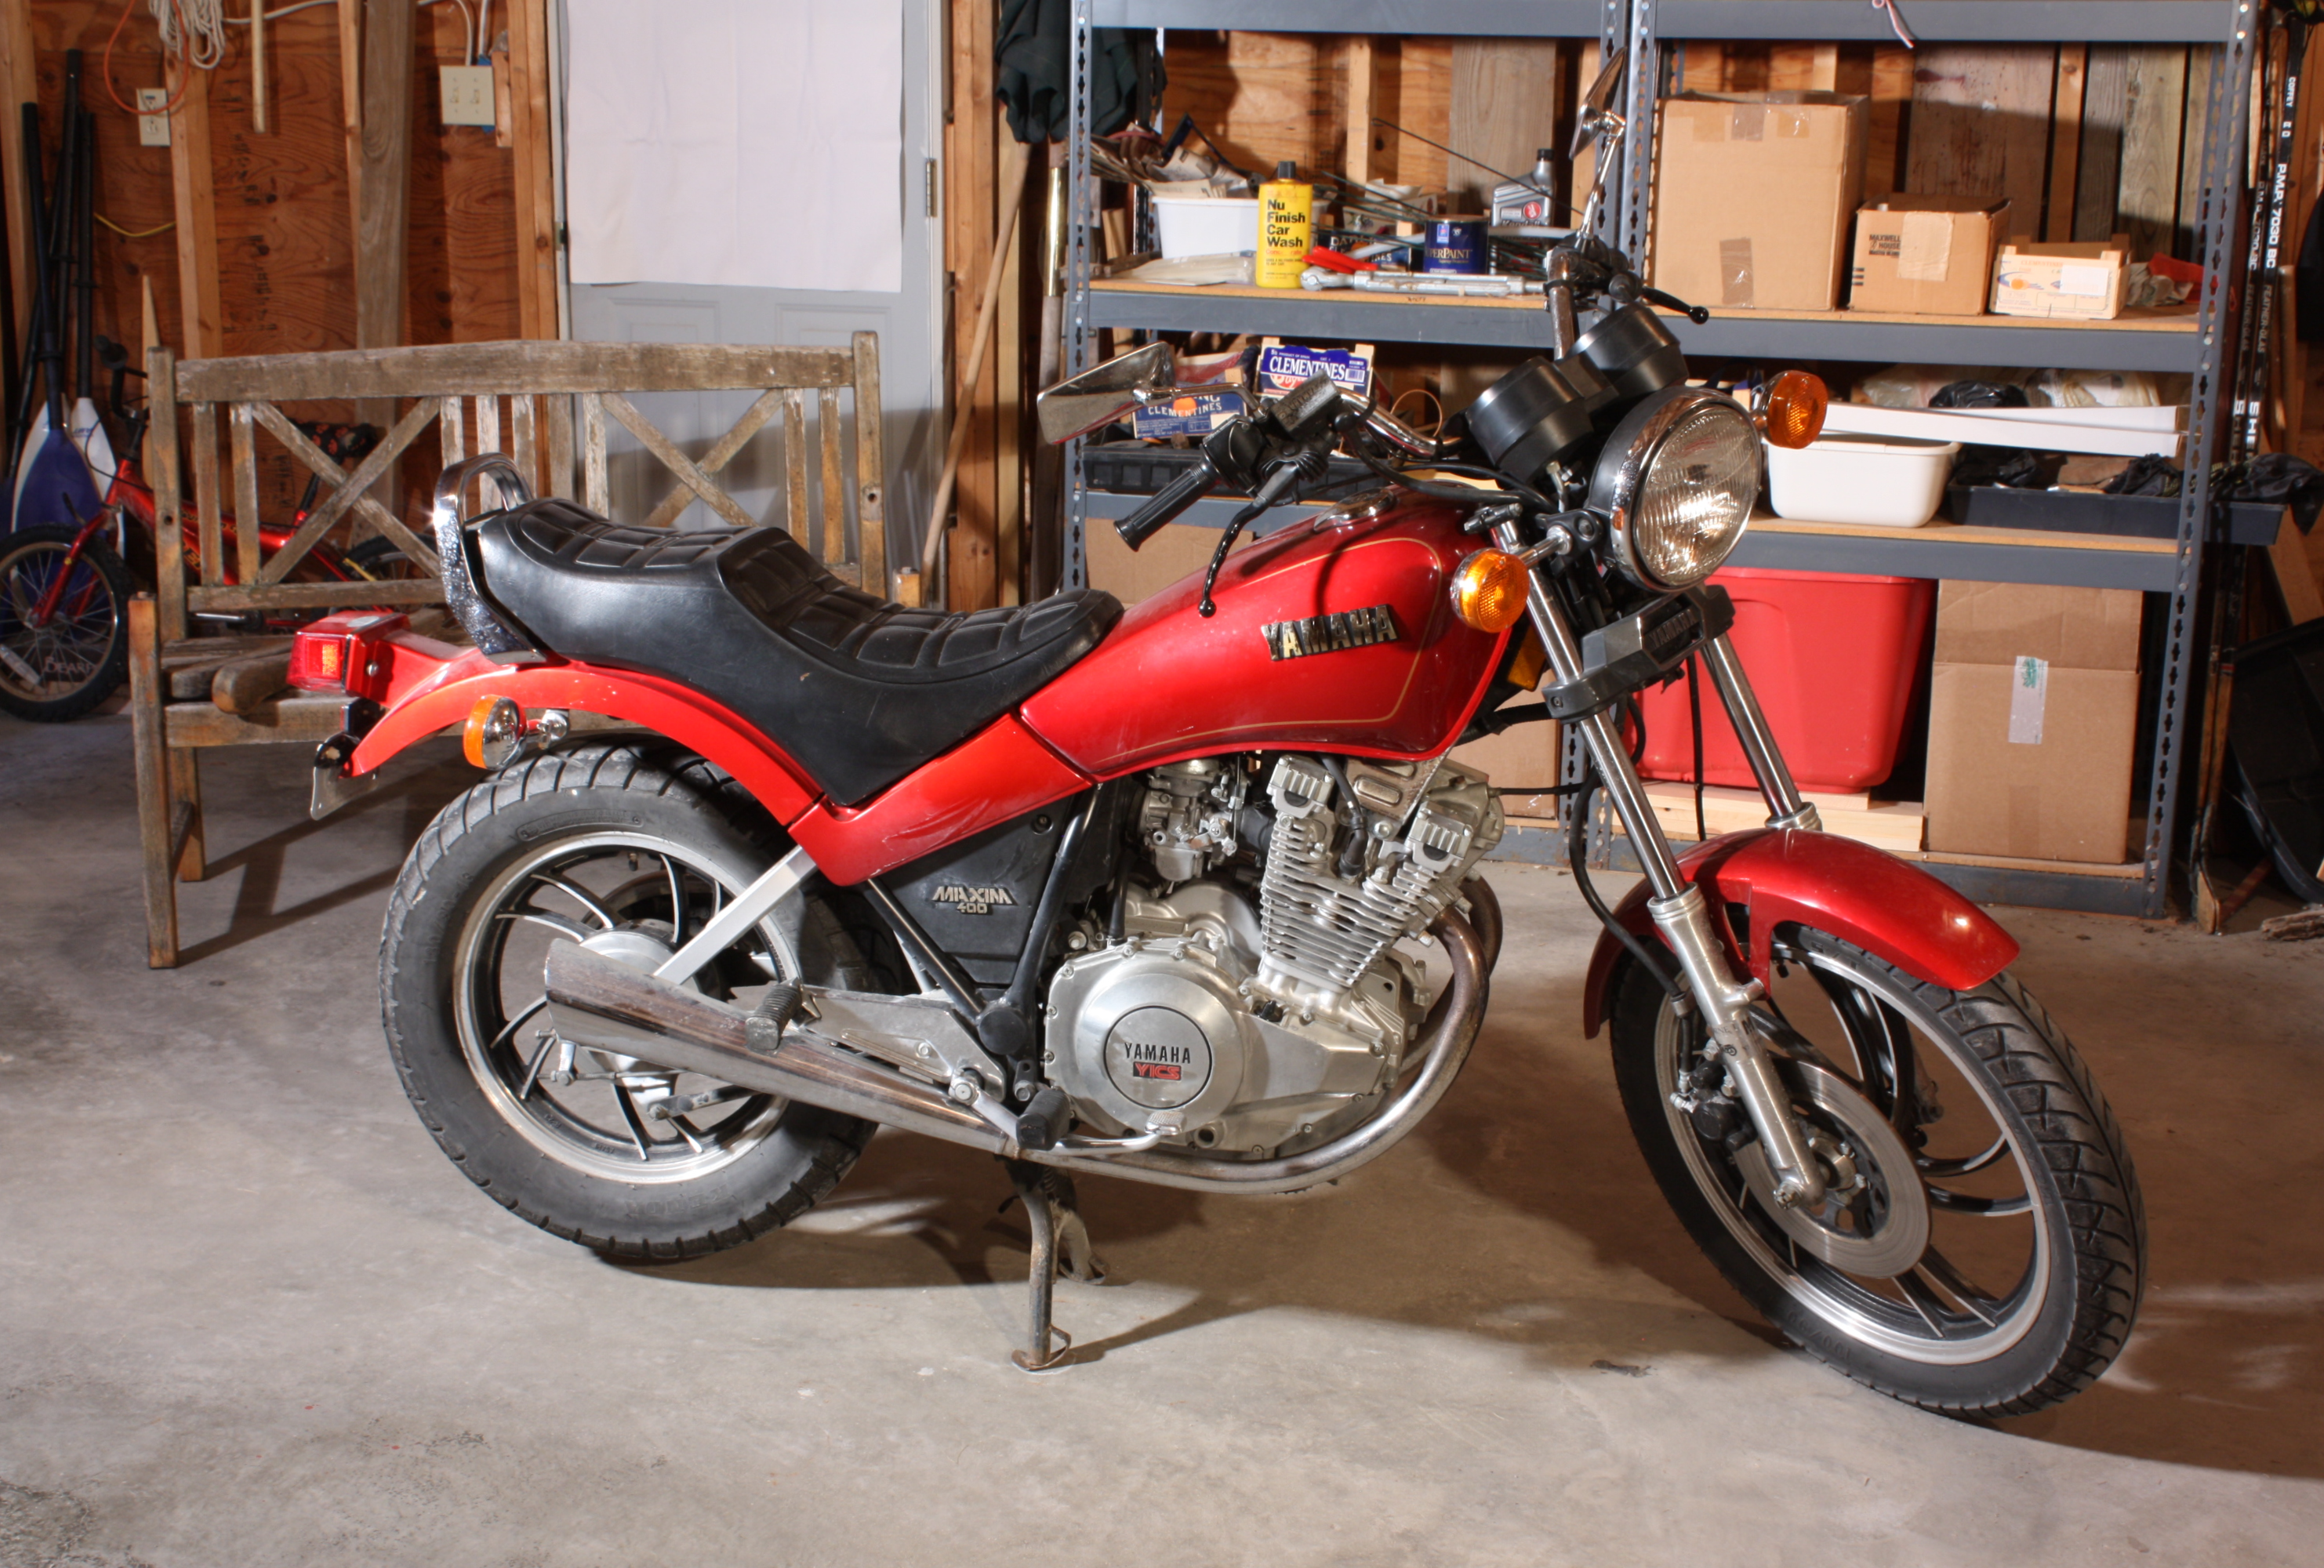
\includegraphics[width=0.4\textwidth]{images/im0.png}
}
	\subfigure[Disparity Left Image Exaple]{
 		 \includegraphics[width=0.4\textwidth]{images/im-0-disp.png}
}
\caption{Middlebury 2014 dataset example}
\label{fig:dataset-example}
\end{figure}

In order to obtain accurate high-resolution stereo datasets, the authors of the described work based their idea on establishing ground-truth disparities from the input views.
In this manner, calibration problem are prevented and the process can be performed via structured light.
However, the drawback of this is that correct disparities can be achieved only for scene points that are non-occluded in both images.
Therefore, extending the idea in \cite{scharstein2003high}, that is based on a self-calibration of structured light sources from initial non-occluded disparities, they managed to register illumination disparities in half-occluded regions and model projector lens distortion as well. 
Moreover, imposing initial correspondences they enhance significantly the rectification accuracy.
Then, subpixel precision was obtained exploiting a high number of binary patterns under multiple exposures and applying a robust interpolation.\\
A brief overview of the pipeline of the process, deeply illustrated in \cite{Scharstein2014}, is now presented.\\

\begin{figure}[t]
	\begin{center}
		\includegraphics[width=.8\textwidth]{images/middlebury-2014-pipeline.png}
		\caption{Pipeline of the overall system for creating the Middlebury 2014 dataset \cite{Scharstein2014}}
		\label{fig:middleury-pipeline}
	\end{center}
\end{figure}

Figure \ref{fig:middleury-pipeline} depicts the overall pipeline of the system defined by Scharstein et al. \cite{Scharstein2014} for reconstruct the stereo datasets.\\
As simply described, the system's inputs are: calibration images of a standard checker-board calibration target; code images obtained with structured lighting projectors from different positions; \textit{ambient} images collected with multiple lighting conditions. 
First of all, re-factoring operations are applied to the unrectified code images, i.e. thresholding, decoding and interpolation.
This leads to floating-point coordinates of the projector pixel illuminating the scene. 
Thus, the achieved values are employed as unique identifiers to impose the correspondences between the two input images. 
So that, the resulting \textit{2D view disparities} are used to refine the \textit{imperfect} calibration in the bundle-adjustment phase.
The next step of the process is use the rectified input images to generate the \textit{1D view disparity}.
The self-calibration of the projector is, therefore, accessed using the merged disparities and thereby produce the \textit{1D illumination disparities}.
View and illumination disparities are, then, combined together into the \textit{perfect} disparities. 
Last row in Figure \ref{fig:middleury-pipeline} shows that rectifying with both calibration allows to achieve the corresponding sets of ambient images.\\
Further details of the single steps of the process are reminded to the original paper \cite{Scharstein2014} so as not to make the discussion much convoluted.\\
Nevertheless, it is worth to disclose that considering the evaluation of the datasets showed in \cite{Scharstein2014}, the choice of the Middlebury 2014 images for the initial tests can be assumed as a correct decision.
As a matter of fact, experimental results reported in the original paper demonstrate how that datasets can be considered highly challenging in terms of accuracy and scene complexity.
Therefore, they can be assumed as a useful starting point for recovering information from the ground truth images available and for the stereo algorithm evaluation.\\




%
\chapter{Methods}
\label{chapter:methods}

A properly planned project requires the analysis of multiple methods and strategies that can be applied during its design. 
Therefore, this chapter displays, focusing on the multiple aspects of the entire project, the different techniques, encountered revising the broad literature accessible in this field, and the decisions that brought to the actual development of the algorithm, which will be thoroughly described in the chapter \ref{chapter:implementation}.\\
In this chapter, an extensive outline of the work made is not produced, though. 
Instead, the following sections focus on a concise, but anyway exhaustive, tracing of the methods available for a correct dense disparity estimation and for image data processing.
Concurrently, the choices made for the specific aspect of the algorithm are defined and explained.

\section{Standard disparity estimation methods}
\label{section:std-methods}

An extensive and broad analysis of the standard and the deep learning methods for dense disparity estimation has already been presented in chapter \ref{chapter:background}, where the review of the literature related to this Master's thesis project has been carried out.
Nevertheless, these sections focus on a different aspect of that analysis, which is correlated to the algorithms that turned out to be the most relevant for this work and to the features of some of the current machine learning based techniques, which appear to be applicable to this project.\\
Considering the standard algorithms for recovering a dense depth image from a stereo pair, the initial approach on which it was decided to focus on for the designing of the project refers to the Semi-Global Matching (SGM) stereo method developed by Hirschm\"{u}ller \cite{Hirschmuller2008}.
The decision of starting to concentrate on that evaluation of the stereo matching problem was mainly driven by the recent methods designed for dense disparity estimation.
As a matter of fact, most of the algorithms created in the last decade are based on the Hirschm\"{u}ller idea or, at least, they make reference to several aspects of the functions outlined in \cite{Hirschmuller2008}.
This fact is clearly comprehensible considering that the SGM method was classified as the best algorithm at the time of its publication and it is currently one of the top-ranked algorithm in terms of sub-pixel accuracy and computational time.
Hence, taking into account the benchmark data based on two of the most employed dataset, i.e. Middlebury \cite{Scharstein2014} and KITTI \cite{geiger2013vision} datasets, and after an initial general review of the literature publish in this field, it results that the top-performing algorithms use key features of SGM in their main pipeline. 
Moreover, it is worth to point out that the majority of the most accurate real time deep learning based algorithm tends to adopt the main functions of the SGM model, exploiting neural networks to ensure real time evaluations of the disparities.
Therefore, it was initially though that a reasonable option for the developing of an algorithm, which would work in real time providing accurate outcomes, would focus the attention of the Hirschm\"{u}ller method.\\
As already introduced in section \ref{sec:stereometh}, the SGM method combines the idea of the standard local based algorithms, where the main cost calculations are made over limited size windows, and global algorithm, for which the best pixel disparity estimation is based on a global energy function. 
Thus, mainly because its hierarchical cost calculation, SGM method outperformed the top-ranked algorithm over the dataset \cite{scharstein2003high}, proving real-time performance of that dataset images. 
However, with the current dataset, such as Middlebury 2014 \cite{Scharstein2014}, KITTI 2012 \cite{geiger2013vision} and KITTI 2015 \cite{menze2015object}, the standard Semi-Global Matching algorithm provide optimal results in terms of accuracy but it tends to slightly suffer if computational time is considered.
For this reason, the most recent real time methods for dense disparity estimation establish the cost computation part of their pipeline over the SGM idea, although, they exploit hardware efficiency or even neural network structures to reach extremely fast computations.\\
Thus, considering this project, it was decided to initially build up the main pipeline on the SGM method structure and employ the stereo device designed by the company to reach real time performances, without loosing in accuracy. 
Furthermore, as previously anticipated, an upstream choice was made. 
As a matter of fact, the current top-performing algorithms strongly depend on convolutional and deep neural network to achieve fast computations.
Contrarily to that, we decided to based the skeleton of our method on the data available through the stereo system to reach a real time implementation.
In this manner, all the problem related to the shifting between synthetic and real environment, faced by deep learning algorithms, would be avoided. \\
The first outline of the algorithm was, hence, partially based on the Semi-Global Matching method \cite{Hirschmuller2008}. 
In order to analyse the suitability of the implementation, absolute computational time performances were not initially taken into account. 
At first it was chosen to focus on the relative efficiency that would be estimated among the different methods used in the principal pipeline.\\
As aforementioned in chapter \ref{chapter:environment}, these preliminary evaluations has been developed in MATLAB. 
In that phase an implementation sufficiently similar to the standard SGM method was designed. 
Thus, the focus was centred on the different types of algorithms used for matching the corresponding pixels and, then, on the part of the pipeline related to the matching and the aggregation costs, as precisely defined by Scharstein and Szeliski in \cite{Scharstein2001}.
The adoption of this working strategy was due to the following motivations. 
First of all, the predominant research aim of this project, whose purpose would most likely further shifts in more market based one, then the need of test the effective performance in accuracy of pure SGM based method and the requirement of analyse the relative efficiency between that algorithm and our method, whose pipeline would be based on the information acquired exploiting the company device. \\
Considering that a fundamental part of this initial testing phase was focused on the matching cost evaluation, multiple matching algorithm has been tested in order to find the most efficient one mainly in terms of accuracy. 
Therefore, basing on the work done in \cite{Hirschmuller2007}, \cite{Patil2013} and \cite{Ko2017}, and making reference to the algorithm used for computing visual correspondence described in \cite{Zabih1994} and \cite{Demetz2013}, the performance of different matching cost algorithms has been analysed.\\

\subsection{Census transform}
\label{subsection:census-transform}

A crucial phase of the SGM algorithm stands in the matching cost computation.
As briefly explained in the background \ref{chapter:background} chapter, this cost is evaluated by computing the difference in the value of intensity among corresponding pixels.
Therefore, especially when dealing with unexpected luminance variation inside the analysed scene, it comes out that non-parametric local transforms are optimal as the support for that correlation \cite{Zabih1994}.
As a matter of fact, these kind of measurements do not rely on the actual intensity values of the pixels, but on the relative local intensities instead.
Therefore, using this kind of models, a considerable number of outliers can be tolerated and improved results are visible especially along object boundaries.\\
Among the commonly used and best performing non-parametric local transform, census and rank transform are described.
Moreover, couple of different implementations of those two classes of transform are introduced.\\
It is widely known in computer vision field that correspondence problem is crucial in depth estimation from stereo pairs.
Correspondence can be, thus, defined by transforming the images with a specific method and then establishing correlations.
In that, the key factor is the transformation, which must tolerate unexpected variation in intensity, for example due to unwanted light source, and in general changes in image bias and gain.\\
Therefore, non-parametric area-based transform rely on local ordering of intensities and not on the actual intensity values.
If an image is considered, and defining as $p$ a random pixel, its intensity becomes $I(p)$. 
Then, let $N_d(p)$ be the set of pixel in a certain square neighbourhood of size $d$, where $p$ is the central pixel. 
Hence, the binary function $\xi(p, p')$ takes value 1 if $I(p') < I(p)$, 0 otherwise.
A non-parametric local transform only rely on the set of pixels in the specific neighbourhood.
Therefore, the \textit{Census transform}, $R_{\tau}(p)$ maps the image subregion surrounding $p$ to an array of bits representing the set of local pixels whose intensity is less or equal than that of $p$. 
Mathematically, the census transform can be formulated as:
\begin{equation}
	\label{eqn:census-transform}
	R_{\tau}(p) = \bigotimes_{[i, j] \in D} \xi(p, p +[i, j])
\end{equation}
where, $N(p) = p \oplus D$, with $\oplus$ is the Minkowski sum and $D$ the set of displacements, and denoting with $\otimes$ the concatenation. 
After the census transform has been applied, the actual comparison among corresponding pixels in done by computing their \textit{Hamming} distance.\\ 
Higher accuracy in corresponding pixel matching can be achieved using an extension of the Census transform, defined as center-symmetric Census transform \cite{Spangenberg2013}.
Therefore, if a square image subregion is taken into account, which has dimensions $n \times m$, we already know from equation \ref{eqn:census-transform} that $s(u, v) = 0, if u \leq v, 1$ otherwise, where now $s( )$ is the sign function.
Precisely, in this notation the census transform can be thus defined as:
\begin{equation}
	\label{eqn:census-transf-2}
	CT_{m,n}(x, y) = \bigotimes_{i = -n'}^{n'} \bigotimes_{j = -m'}^{m'} s(I(x, y), I(x + i), y + j)
\end{equation}
where $n' = [n/2]$, and $m' = [m/2]$.
Hence, as shown in Figure, the center-symmetric census transform can be mathematically defined as:
\begin{equation}
	\label{eqn:center-symmetric-census}
	CS-CT_{m,n}(x, y) = \bigotimes_{(i, j) \in L} s(I(x - i, y - j), I(x + i, y + j))
\end{equation}
where $L = L_1 \cup L_2$, $L_1 = R_{-n',0} \times R_{-m',0} \setminus {(0, 0)}$, $L_2 = R_{1,n'} \times R_{-m',1}$ and $R_{a, b} = {x \in \mathbb{Z} \vert a \leq x \leq b}$.
Because, only center-symmetric pairs of pixels are compared, the formulation in equation \ref{eqn:center-symmetric-census} needs less bit than the one in \ref{eqn:census-transf-2} to describe the same patch. 
As aforementioned, the actual matching cost is then computed using the Hamming distance between corresponding pixels. 

\subsection{Rank Transform}
\label{subsection:rank-transform}

\subsection{Conventional intensity based methods}
\label{subsection:conventional-methods}

\section{Deep-learning based methods}
\label{section:deep-learning-method}




\section{Pure derivative based data estimation algorithm}
\label{section:deriv-based-algorithm}

\section{SGM based data estimation algorithm}
\label{section:sgm-based-algorithm}


\section{Pre-processing techniques}
\label{section:pre-process-tech}

\section{Post-processing techniques}
\label{section:post-process-tech}


% 
\chapter{Algorithms implementation}
\label{chapter:implementation}

The actual implementation of the designed algorithms introduced in Chapter~\ref{chapter:methods} is now extensively described. 
As anticipated in the previous chapter, here all the details of the developed phases of the project are deeply analysed and explained. 
A path similar to the one followed during the actual designing of the algorithms is used for outlining the whole project.\\
First of all, the preparatory tests performed for evaluating the feasibility of the conceived idea are reported and explained. 
Subsequently, the focus moves on the two main methods designed, the derivative based one and the strategy based on the standard SGM pipeline.
After that, the side phases of the work are presented. 
The pre and post-processing operations are accurately defined and the comparison among the different filtering operations are carried out.

\section{Preparatory and testing phase on MATLAB}
\label{section:prep-pahse-matlab}

\begin{figure}[t]
	\centering
	\subfigure[Left ground truth stereo test image overlapped by a simulated point grid]{
 		\includegraphics[width=0.4\textwidth, height= 5cm, keepaspectratio]{images/disparity-plus-grid-test-left-01.png}
 		\label{fig:test-matlab-left-01}
}
	\subfigure[Right ground truth stereo test image overlapped by a simulated point grid]{
 		 \includegraphics[width=0.4\textwidth, height= 5cm, keepaspectratio]{images/disparity-plus-grid-test-right-01.png}
 		 \label{fig:test-matlab-right-01}
}
\caption{Ground truth images from the Middlebury dataset used for the initial testing phase}
\label{fig:test-matlab-01}
\end{figure}

As anticipated in Chapter~\ref{chapter:methods}, the first phase of the project can be mainly considered as a researching stage.
As a matter of fact, exploiting the stereo images from the Middlebury 2014 dataset, some tests have been performed to obtain an estimation of the feasibility of the conceived idea.\\
Therefore, as Figure~\ref{fig:test-matlab-01} displays, ground truth images have been initially used.
Thus, a point grid, similar to the one generated with the LadiMo device, has been simulated and overlapped to the input images.
In particular, as the difference between Figure~\ref{fig:test-matlab-left-01} and Figure~\ref{fig:test-matlab-right-01} illustrates, to have a reliable simulation of the 3D point cloud generated by the device, the only grid that was actually defined was the one over the principal image, i.e. the left one.
As a matter of fact, as defined in section~\ref{section:stereo-device}, the hardware exploited in the project is provided with only one laser projector.
Therefore, this allows to utilize the produced point cloud only over one image\footnote{Technically speaking the initial cloud of point created through the device can be independently related to both of the image, depending on which is used as the reference one, just applying the correct transformation between the laser and the principal image coordinates systems}.
After that, those input data, together with the grayscale stereo pair, have been employed in a stereo matching pipeline to recover a disparity map of the analysed scene.\\
In order to acquire useful baseline data regarding the practicability of the thought strategy, tests and analysis over the different areas of the main loop of the algorithm have been investigated.
Actually, this research has been performed with a precise method. \\
First of all the stages of a standard stereo matching method, as defined by Scharstein and Szeliski in~\cite{Scharstein2001}, have been separately examined. 
Thus, in order to do this in a reasonable way, the literature regarding both standard and novel stereo matching algorithm has been studied and the main features of the designed algorithm checked out. 
As an example, if the matching cost phase is taken into account, different approaches are presented in the literature for evaluating the similarity among the image pixel values for the respective disparity levels. 
As a matter of fact, as introduced in Chapter~\ref{chapter:methods}, the Hamming distance between corresponding pixels can be exploited to determine that measure. 
In relation to that, different algorithms exist to apply a transformation to the input images, making them available for an appropriate implementation of the aforementioned matching cost calculation.
For the actual tests carried out, local methods have been mainly analysed, being more appropriate for the type of data available and for the purposes of the designed strategy.\\
Therefore, as matching cost measures, simple operations have been initially taken into account, such as the sum of absolute differences (SAD) and the sum of squared differences (SSD). 
Moreover, more accurate methods have been later evaluated, i.e. the Rank transform, and its improved version, the Complete Rank transform, broadly discussed in~\cite{Demetz2013}.
Then, the Census transform and the Center-Symmetric Census transform proposed by Spangenberg et al. in~\cite{Spangenberg2013} have been investigated.
Considering all of those algorithm, it resulted that the most suitable methods are equivalently the Rank and the Census transform.
In fact, being these non-parametric transformations, they are not sensitive to changing in lightning inside the environment, thing that usually happen when managing real industrial areas. 
Considering that, at the end the Center-Symmetric Census transform has been chosen because of its reliability, which is comparable to the aforementioned methods, and for the fact that it uses a lower amount of bits to describe the single pixel value compared to the standard Census transform.\\
During this phase of testing, the decision was to run a single pipeline of an \textit{SGM-based} algorithm, whose aggregation cost phase would be based on the four orthogonal directions. 
Moreover, another operative choice was to use the whole image for the complete execution of the designed method.
Therefore, it was thought that, at least for this researching phase, it would be meaningless to define a hierarchical implementation of the code, where the image is initially downscaled and subsequently scaled up again in order to make the execution faster, as made by Hermann and Klette in their application of the SGM algorithm~\cite{Hermann2013}.\\
At the end of this \textit{research} section of the project, the results did not show an exact path to follow, meaning that there was not a clear improvement over the normal SGM-based approach by using the initial set of grid point, compared to the MATLAB built-in method used as baseline. 
Specifically, the disparity image obtained was actually lower in accuracy compared to the method implemented in MATLAB by Eric Psota and available at the website of the Middlebury stereo dataset \footnote{\href{http://vision.middlebury.edu/stereo/submit3}{links Middlebury College Stereo}} and to the MATLAB built-in method \texttt{disparitySGM()}. 
Moreover, the developed implementation was quite slow, if correlated to the benchmark of most of the standard SGM-based methods. \\
However, some considerations should be proposed regarding that outcome. 
First of all, the algorithm designed runs iteratively, that is no parallel loop is coded to make the execution faster.  
This is, in fact, explained by the decision of being interested in the relative performance among the own designed methods. 
Furthermore, any sort of GPU enforcing was not used. 
Hence, it was quite expected to not obtain good performance.
Therefore, the thought strategy was evaluated as feasible and, additionally, the exploiting of proper initial data provided by the stereo camera would likely be an enhancement to the overall performance of the algorithm. 
Moreover, the derivative based algorithm has not been initially tested, however, considering its main idea, it should theoretically give accurate results in a reasonable computational time.

\section{Derivative based method implementation}
\label{section:derivative-based}

Verified the feasibility of the considered strategy, the project design shifted to the actual algorithm development. 
Therefore, exploiting the OpenCV libraries and using the images from the Middlebury 2014 dataset, the derivative based method started to be implemented in a C++ code. \\
In the initial phase of its designing, the simulated grid based on the ground truth images was still used to obtain the input point cloud data.
As a matter of fact, the only practical advantage of employing such simulated data stands on the amount of noise that they contain.
As a matter of fact, an appropriate comment to that strategy would be that, once the real data from the device would be used, the result would probably be worse in terms of overall accuracy. 
Anyway, at that initial stage of the algorithm development, the interest was focused on comparing the performance of the pure SGM-based and the derivative-based implementations. 

\subsection{General features of the method and simulated grid specifications}
\label{subsection:general-feature-der-method}

\begin{figure}[t]
	\begin{center}
		\includegraphics[width=.8\textwidth, height=5cm, keepaspectratio]{images/grid-subwindow-detail}
\caption{Detail of a point grid patch where a set of neighbouring points is highlighted}
\label{fig:grid-subpatch}
	\end{center}
\end{figure}

\begin{figure}[t]
	\begin{center}
		\includegraphics[width=.8\textwidth, height=5cm, keepaspectratio]{images/point-estimation-detail}
\caption{Detail of a point grid patch where the estimation of a new point at relative coordinates $i$ and $j$ is performed}
\label{fig:subpatch-estimation}
	\end{center}
\end{figure}

The so called derivative-based method, which arises to be both efficient and generally accurate, based its strength on the sparse point cloud gained through the structured light assisted stereo camera.\\
The main features of that algorithm are now precisely described.
Moreover, attention is focused on the conventions utilized to define the main parts of the method and on the functions created for obtaining the 3D point estimations over the initial laser grid. 
Subsequently, some fundamental sections of the designed implementation are more broadly described, thus to provide to the reader a complete understanding of the work done. \\
For this reason, the analysis starts by considering a simulated grid of points, which was defined in the C++ code in order to initially mimic the real laser grid generated by the LaDiMo device. 
In fact, the actual grid of points generated by the company device is not perfectly parallel to a vertical plane, as the simulated one, contrarily it is tilted at $16.7^{\circ}$ w.r.t. the vertical axis.
However the approach followed, as aforementioned, does not invalidate the outcome obtained through all the designing process of the method.
Instead, it is a reasonable strategy for achieving some initial temporary results, which can then provide a guidance to the following phases of the whole process.\\
Therefore, let us consider the entire point cloud as a regular grid where each point is defined by its coordinate in space.
Additionally, it can be also thought that the corresponding 2D coordinates in the reference image plane can be easily retrieved using the camera projection matrices.
Hence, if a neighboring set of four points is taken into account, as highlighted by Figure~\ref{fig:grid-subpatch}, the local derivative vectors for all the considered coordinates can be easily calculated.
This estimation of the derivative is extremely useful for the following reasons.
First of all, they are, actually, exploited to generate the estimations inside each grid sub-region.
Moreover, they can be employed to evaluate if, inside the specific patch of points, there could be an edge of some shape. 
In this latter case, the magnitude of the $Z$ component of the derivative vector will, in fact, be higher than a set threshold, which can be defined looking at the average values of the $Z$ coordinate of the grid points.\\
Therefore, explaining the project design procedure implemented, it can be summarized as follows.
Initially, for each one of the points in the grid the internal and external derivatives have been calculated with respect to its four neighbors, as the arrows in Figure~\ref{fig:grid-subpatch} underline. 
This means that each point will have, then, four distinct set of local derivatives, for both the internal and the external ones, conventionally defined as follows:
\begin{itemize}
	\item \textbf{from top:} derivative between the specific point and its top neighbor;
	\item \textbf{from boottom:} derivative between the specific point and its bottom neighbor;
	\item \textbf{from left:} derivative between the specific point and its left neighbor;
	\item \textbf{from right:} derivative between the specific point and its right neighbor.
\end{itemize}
In these definition a neighbor to a point is defined with the subsequent rule. 
Let us consider a point, which is classified through the grid coordinates $r$, along the row grid direction, and  $c$, along the column direction. 
Its neighboring points are, hence, identified by:
\begin{itemize}
	\item \textbf{top} neighbor: with coordinates $r - 1$ and $c$;
	\item \textbf{bottom} neighbor: with coordinates $r + 1$ and $c$;
	\item \textbf{left} neighbor: with coordinates $r$ and $c - 1$;
	\item \textbf{right} neighbor: with coordinates $r$ and $c + 1$;
\end{itemize}
Using that scheme the four derivatives estimated for each point will contain the difference between the actual point  \textbf{\textit{full location components}} and the ones of the relative neighbor regarding.
In the implemented code, the introduced \textbf{\textit{full location components}} are in the order: the $X$, $Y$ and $Z$ space coordinates of the point, in meters, the $x$ and $y$ components of the point projected in the principal image plane, therefore they are measured in pixels, and finally, $d$ is the disparity value, in pixel, related to the depth of the point, which can be evaluated through equation~\ref{eqn:disparity-depth} and adding the relative \textit{disparity offset} if required.
This gain was, in fact, necessary when using the data from the Middlebury dataset, where the relation between the ground truth disparity values and the corresponding depths is defined as in the equality~\ref{eqn:middlebury-depth-disp}
\begin{equation}
	\label{eqn:middlebury-depth-disp}
	Z = \frac{B \cdot f}{d + d_{offs}}
\end{equation}
where, as in~\ref{eqn:disparity-depth}, $B$ is the camera baseline, $f$ the respective focal length and $d_{offs}$ the disparity offset, which is the different between the $x$ coordinate of the principal points, as following clarified:
\begin{equation}
	\label{eqn:doffs-equality}
	d_{offs} = c1_x - c0_x
\end{equation}
where $c1_x$ is the $x$ coordinate of the principal point for the support camera, while $c0_x$ is the $x$ coordinate of the principal point for the main camera.\\
Therefore, let us now consider to estimate an unknown point inside a subregion of the whole grid, that was decided to be identified by 4 points, as Figure~\ref{fig:subpatch-estimation} displays.
The final 3D coordinates of the new point will be, at first, defined by four different estimations, each one related to the four corners of the grid subwindow, as follows.

\begin{subequations}
\label{eqn:point-patch-estimation}
	\begin{align}
		est_{TL} = TL + i \cdot der_{from-left} + j \cdot der_{from-top} \\
		est_{TR} = TR + (i-1) \cdot der_{from-right} + j \cdot der_{from-top} \\
		est_{BL} = BL + i \cdot der_{from-left} + (j-1) \cdot der_{from-bottom} \\
		est_{BR} = BR + (i-1) \cdot der_{from-right} + (j-1) \cdot der_{from-bottom}
	\end{align}
\end{subequations}

where $TL$, $TR$, $BL$ and $BR$ respectively point to the estimation done with respect to the top-left corner of the grid sub-window, the top-right corner, bottom-left and bottom-right corner. 
Then, $i$ and $j$ are the relative $x$ and $y$ coordinates of the estimated point, whose values range between 0 and 1.
Finally, in the notation employed, $der_{dir}$ stands for the different derivative vectors related to each corner point and visualized by the arrows in Figure~\ref{fig:subpatch-estimation}.
Here, in order to keep the generality of the notation, no distinction has been made between internal and external derivatives.
As a matter of fact, in both cases the calculation performed are actually the same.
The difference only interests the specific values of the vectors and the analysed case, considering that the internal derivatives are in general used.
The external ones are exploited when some sort of edge is detected inside the analysed patch, after having verified that other edges are not located on the close neighborhood of the targeted subwindow. \\
Once, these estimations are achieved exploiting the derivatives, as equations in~\ref{eqn:point-patch-estimation} define, the best evaluation is obtained by calculating each matching cost between the corresponding pixels between the stereo images. 
The matching cost is determined following the subsequent routine.\\
In relation do this, it should be reported that, due to the researching aspect of this project, lots of changing have been made to the code.
Therefore, to provide a clear explanation of the decisions made and the procedure followed, which, otherwise, could appear somehow winding, all the relevant changes to the functions used are disclosed. 
Beside this brief comment about the designed code, the best, among four, estimation of the new grid point is such evaluated.\\
The estimation provides the values of the 3D coordinates of the calculated point and its disparity.
The point location is, then, projected through the camera matrix to the reference image (usually the left image) pixel coordinates and the corresponding position in the support image is determined using the estimated disparity value. 
At this point the matching cost is computed as the absolute difference between the intensity values of the analysed pixels in the left and in the right image planes. 
However, this kind of measure appears to give weak results. 
As a matter of fact, the main problem was that, in some situations, the estimation labelled as the best one actually contained a value of disparity doubtful, if compared to the one of the point's closest neighbors.  
Moreover, this generally happened in texture-less regions, where it is obviously more difficult to make accurate estimations.\\
To overcome this problem, a penalty value was added to each partial estimation. 
Specifically, that value was weighted linearly basing on the distance between the estimated point and the corresponding corner. 
In this manner, the estimation, related to the disparity and to the coordinate values of the closest corner, is most likely to be addressed as the best one.
Once the best estimation for each new point is calculated, the evaluated values of the 3D point coordinate are processed, applying a morphological filter, in order to remove undesired noise and smooth out the overall data. \\
The estimation procedure just described is not actually able to handle all kind of situations, concerning the provided input objects.
In fact, incorrect values used to be estimated in subregions affected by edge features, and thus occlusions. \\
Therefore, to correctly manage these situations, multiple cases have been defined, regarding the edge cases. 

\subsection{Edge cases and penalty values discussion}
\label{subsection:edge-cases-and-penalties}

At first, four main conditions have been distinguished. 
These comprise the possibility to do not have any type of edge inside a grid subregions, the existence of a vertical edge in the patch, an horizontal edge case and finally a so called \textit{undefined} case has been defined.\\
Therefore, in each one of these situations, the point estimation procedure differs slightly, so that the aforementioned linear penalty can be more wisely set.
Regarding this two distinct values of the penalty have been employed, a lower and a higher value.
In fact, because it is not efficiently possible to correctly estimate the position of the potential edge, the choice of the correct estimation has to be somehow driven by exploiting the linear penalties. \\
Moreover, to identify the correct type of edge, the derivatives have been exploited and, specifically, the magnitude of the $Z$ component of the vector. 
Basically, a general edge case, which is equivalent to the \textit{undefined} condition, is initially verified by computing the absolute difference between the $Z$ components of all the possible couples of corners, i.e. the $Z$ value of the local derivatives, and comparing that with a pre-determined threshold, which is related to the average depth value of the initial points of the grid. \\
Therefore, during the algorithm pipeline, the possibility of having an edge feature inside the specific patch is initially checked.
Then, if the depth values of the four corner are almost equivalent, this means that the area is actually planar.
Thus, in this situation, a fast interpolation method is run, so that the overall computation can be even faster.\\
On the contrary, if a vertical or an horizontal edge is found, the small and big penalties are used accordingly.
For example, if the edge is vertical, the small penalty will be multiplied to the relative $y$ coordinate of the estimated point, instead the big penalty will weight the $x$ coordinate.\\
Finally, for the undefined case, the penalty weight is equivalent in both directions, $x$ and $y$, and its magnitude ranges between the two previously defined values. \\
Those three different edge cases are the one initially tested. 
However, later appeared that a more meaningful strategy should be based on the definition of two grater categories, which would comprise the cases described above.
These two bigger classes describe, thus, \textbf{\textit{soft}} and \textbf{\textit{strong}} edges. 
In fact, results of tests done with dataset images show that employing a single threshold for the depth difference and focusing only over the edge direction was not entirely adequate. 
As a matter of fact, in a generic scene different types of objects exists. 
Therefore, adapting the edge analysis to the object distances, for example between the whole foreground and the background and between multiple objects of the foreground, that would give a smoother and more accurate final dense 3D point cloud.

\subsection{Derivative computation and sanity check}
\label{subsection:derivative-computation}

The core of the estimations are, actually, the local derivatives computed for each point of the grid. 
Basically, each grid point contains four vectors, which are the local derivatives between the reference point and its four orthogonal neighbors. \\
Initially the mere derivatives have been calculated as pointing towards the reference point, like Figure~\ref{fig:grid-subpatch} shows. \\
However, it came out that this procedure was not enough accurate, to generate a proper dense 3D point cloud.
Therefore, a \textit{sanity check} has been later defined inside the derivative calculation pipeline to achieve preciser computation of the local derivatives, especially for the grid sub-patches where edges are most likely to be found.\\
Moreover, a higher accuracy of the final result has been achieved when evaluating, for each grid point, two slightly different types of derivative vectors.
Specifically, \textbf{\textit{internal}} and \textbf{\textit{external}} derivatives. 
This distinction allowed to achieve faster and more accurate results, especially when dealing with edges in the grid subregion. 
Precisely, if the presence of an edge is verified for the considered patch, the external (with respect to the sub-window) derivatives were used.
Otherwise, exploiting the internal derivatives the computation could be made faster, being them equal in couple among the corners of the patch. \\
Referring to what introduced at the end of Section~\ref{subsection:edge-cases-and-penalties}, in the latest implementation designed, the estimation process is mainly driven by the edges analysis. 
As aforementioned, the test results demonstrate that a distinction based only upon the edge shape is not enough to reach a good degree of accuracy.
Therefore, the analysis cases have later been defined basing on the strength of the edges between the objects in the scene.\\
Hence two different thresholds have been so determined. 
The first is used to identify occlusions that basically occur between foreground objects and the background. 
These have been designated as \textbf{\textit{strong}} edges. 
Differently, the other case is specified as the \textbf{\textit{soft}} edges case.
This is related to occlusions happen between parts of the same object at different values of depth, as could be between the chin and the neck of a person.\\
Moreover, on top of this first level of edge selection, the following cases have been then defined, which are correlated to the specific value of the penalty.
Precisely, they are \textit{pure vertical} and \textit{pure horizontal} edges, for which it should happen that the depth values of the corners are equals in couple.
Then, there are some particular cases, which have the scope of leading the disparity estimation to a higher level of accuracy.
They are: \textit{diagonal top left}, \textit{diagonal top right}, \textit{diagonal bottom left}, \textit{diagonal bottom right}.
Furthermore, there is the undefined case, which is triggered when the potential edge found in the subregion has a strange shape.\\
Taking now into account the actual estimation functions, these are slightly different for the aforementioned edge cases identified.
Summing up the overall procedure, it can be said that, the main distinction, which guides the whole process is the first one, that is the one that distinguish among, strong, soft and no edges.
Then, for all the subcases, the main difference stands on the values and order of the penalties. \\
Hence, in the \textit{no edges} case, four temporary estimations are performed for each new grid point by carrying out a linear interpolation, which exploit the \textit{internal} derivative vectors.
Then, for the other two main cases, the procedure is generally the same. 
In fact, the fundamental scope of distinguish between those types of occlusions is to make the final outcome smoother. \\
Thus, when dealing with edges, at first the algorithm checks for each temporary estimation, that is for each subregion corner, if there could also be edges in the neighborhood outside of the region. 
If this is false, a linear interpolation is computed employing the \textit{external} derivatives.
Otherwise, the interpolation is done with the \textit{internal} derivatives and only for the $x$ and $y$ pixel positions. 
Instead, the depth value is matched with the one of the corresponding corner, thus to enhance the smoothness of the final result.
Regarding the $X$, $Y$ and $Z$ values, these can be easily recovered from the previously estimated pixel coordinates and disparity, by exploiting the camera projection matrices and the relative equations. 

\section{Semi-Global Matching based method implementation}
\label{section:sgm-based}

The other implemented method based on the initial grid of points follows more closely the standard stereo-matching structure.
Moreover, it does not distinguish between \textbf{\textit{strong}} and \textbf{\textit{soft}} edges, but the different cases are identified only considering the shape of the potential edge present inside the subwindow. \\
Therefore, this algorithm initially computes the \textit{matching cube cost} for the specific grid patch. 
The difference between the standard SGM method stands on that cube, whose third direction does not generally contains continuous values of the disparity.
On the contrary, those values are defined by the sub-window corners, whose disparity define the levels of the cost cube.\\
Therefore, if no edge is found, only the matching cost part of the stereo algorithm is carried out.
Otherwise, the aggregation cost phase is implemented.
In this latter case, the cost is actually aggregated only on the direction orthogonal to the shape of identified edge, thus to make the implementation faster.
As a matter of fact, let us consider a specific sub-patch in the principal image and the pixels that belong to it.
Let us, then, assume to identify a vertical edge inside that subregion.
It would be worth nothing to aggregate the matching costs related to each pixel along the vertical direction.
The differences among the intensity values of the pixel along that direction would, in fact, be extremely lower than the variations along the orthogonal direction.
Therefore, because in general the matching costs are aggregated along all of the four orthogonal directions, the values along the path orthogonal to the edge will weight more.
While the costs along the path parallel to the edge will have less relevance, technically speaking.
Therefore, it would be worth nothing to aggregate the cost along all the four directions, obtaining as the only outcome an increasing in the algorithm complexity.
On the contrary, if a particular edge is determined inside an image patch, it would be more efficient to run the aggregation cost step along the two orthogonal directions only.\\
At the end of the pipeline simple post-processing operations are performed over the obtained data, as done for the other algorithm.
Considering the overall method, it result to be give a denser point cloud compared to the previous method. 
However, its computational time is extremely higher.
This is clearly due to the fact that this algorithm estimates each single pixel inside the specific subregions.
Contrarily, in the \textit{lightweight} strategy the number of samples that the user wants to estimate can be adjusted. 
In this way the trade-off between accuracy and resources utilization can be externally defined. 

\section{OpenCV built-in Semi-Global Box Matching algorithm}
\label{section:opencv-sgm-method}

\section{Pre-processing testing and analysis}
\label{section:pre-processing-impl}

The pre-processing phase can be ideally divided in multiple parts.
First of all, general operations have been applied for both estimation methods in order to remove noisy components from the stereo pair and from the ground truth images, when exploiting the simulated grid for the estimations.
Then, a section of the pre-processing phase can be considered the importing of all the necessary calibration data and the creation of a sort of look-up table, which was used together with the grid of points.\\
On the contrary, when working with the real data coming from the LaDiMo stereo device, some initial operations have been necessary to clean up \textit{bad} point values and for estimating some of the missing data, which would be determined without losing in accuracy. \\
Regarding the image pre-processing, different noise removal filters have been tested over database images, in order to understand which would provide the best trade-off in most of the cases. 
Median and bilateral filters appear to be, almost equivalently, the best choice for smoothing away the noise while loosing the smallest amount of information from the input images, because of the peculiarity of being edge preserving filters. \\
Considering the others pre-processing operations implemented in the algorithm, they depend on the condition of working or not with the simulated grid.

\subsection{Look-up table and point grid pre-processing}
\label{subsection:grid-preprocessing}

Therefore, for the initial testing phase of the algorithm designing, when multiple tests have been carried out using the images from the Middlebury dataset, a look-up table has been defined in order to ensure a fast data retrieving. 
This structure has been easily built by progressively numbering the simulated gridpoints, so that their values correspond to the row index of the \textit{complete data matrix}.
That is the matrix that actually contains the space and relative pixel information for all the point belonging to the initial grid, i.e. $X$, $Y$ and $Z$ in meters or millimetres and $x$, $y$ and \textit{disparity} in pixels. \\
Regarding the implementation run over the real data, instead, some pre-processing operations have been necessary to adjust the initial device data, which were not always perfect. 
As a matter of fact, a low percentage of points of the laser grid, which ranges between 2.7 and 3.2 \% depending on the specific scene (\textbf{check the error percentage, not sure}), was missing. 
It used to happen that the points were, in fact, not visible in the grid, as overlapped to the raw image, however, the raw data coming from the device present their grid coordinates alone, without any further information about their location.
Therefore, those points were labelled and ordered by the algorithm running on the device, however no data were available regarding their space or image positions.
This behaviour usually happened for the points located close to edges, and thus close or even above occlusions. 
In those cases the accuracy of the device drops locally and the provided results are, in fact, missing. 
So that, pre-processing procedures were necessary in order to reduce the percentage of initial errors, which usually diminishes between 0.8 and 1.2 \%, depending on the density of missing data in the occluded regions.
However, even if in general the error dropping was not high, it marginally impacts on the overall performance of the algorithm, providing more accurate results in regions interested by edges and, hence, occlusions. \\
Specifically, two main operations have been performed over the initial raw data to reduce the errors.
First of all, the grid points have been entirely analysed in order to identify the area where the percentage of missing data were low enough to allow a highly accurate reconstruction of the values of those point.
As a matter of fact, a non perfectly exact estimation would carry errors over all the algorithm pipeline, which is a not desirable outcome. \\
Hence, where enough raw data were present in the neighborhood of occlusions, the estimations have been performed by evaluating a fast yet accurate linear interpolation exploiting the four closest neighbors to the specific point. 
Related to this, it was proved that performing a bilinear interpolation or using a weighted average to estimate missing values had the same grade of efficiency as the simple average, employing at least two orthogonal neighbours. \\
After the data filling a minor percentage of missing values was generally still present. 
Therefore, before running the algorithm those grid points was removed, being useless in the whole pipeline.
In regard to this, it is worth to make notice that the \textit{bad} points were in most of the cases almost the 2.5 - 3 \% of the entire grid data. 
Therefore, it can be concluded that the value would not affect sensibly the overall accuracy of the final result and that a high density of point could be certainly reached with the available amount of raw data.\\
On the other hand, the application of a high expensive method, which would probably only provide an additional error reduction of the 0.5 \% would be worth noting and it would most likely affect the speed of the algorithm, without providing a reasonable improvement of the density of the final point cloud.
Therefore, it was considered beneficial to apply the aforementioned data recovering, over the condition of filling the missing data with a high accuracy. 
Considering, in fact, that the initial amount of errors was generally acceptable for achieving final accurate results, a mild data retrieving, which would not affect the performance of the algorithm while slightly increasing the amount of initial information, has been evaluated as valuable for the whole method.

\subsection{Image undistortion and rectification}
\label{subsection:img-undist-and-rectific}

\begin{figure}[t]
	\centering
	\subfigure[Left distorted raw image]{
 		\includegraphics[width=0.4\textwidth, height= 5cm, keepaspectratio]{images/input-image-raw-left.png}
 		\label{fig:distort-raw-left}
}
	\subfigure[Right distorted raw image]{
 		 \includegraphics[width=0.4\textwidth, height= 5cm, keepaspectratio]{images/input-image-raw-right.png}
 		 \label{fig:distort-raw-right}
}
	\subfigure[Left rectified stereo image]{
 		\includegraphics[width=0.4\textwidth, height= 5cm, keepaspectratio]{images/output-image-rect-left.png}
 		\label{fig:stereo-rect-left}
}
	\subfigure[Right rectified stereo image]{
 		 \includegraphics[width=0.4\textwidth, height= 5cm, keepaspectratio]{images/output-image-rect-right.png}
 		 \label{fig:stereo-rect-right}
}
\caption{Distorted raw and stereo rectified images from the Ladimo device}
\label{fig:stereo-undist-rect-4eye}
\end{figure}

Concerning the tests carried out with the real environment images taken from the LaDiMo device, some pre-processing was necessary on the stereo pair too. 
In fact, the hardware employed gives as an output, on top of the point cloud data, a pair of distorted raw RGB images, which has to be first undistorted and then rectified, in order to be correctly used for the stereo matching. \\
Specifically these operations have been completed using the OpenCV built-in functions \texttt{stereoRectify()}, \texttt{initUndistortRectifyMap()} and \texttt{remap()}, which employ the camera calibration data, already available for the used camera, and give as output the matrices that map an image from the distorted reference systems to the stereo rectified space.
In this section a concise explanation of the chain of operations that has been implemented with those functions is proposed.
If further details regarding the specific parameters correlated to those functions are needed, the broad OpenCV documentation available is reminded.\\
Firstly the \texttt{stereoRectify()} function is fed with the original camera matrices and the distortion parameters of the two camera, which are available from the pre-computed calibration procedure.
Moreover, as input to the function there is the transformation matrix from the coordinate system of the principal camera to the secondary camera.
Actually, that is provided as the rotation matrix and the translation vector separately.
Hence, the OpenCV function provides as its main outputs the two rectification transform matrices, that are the matrices that bring the 3D coordinates of a point from the unrectified coordinate system to the rectified coordinate system.
Moreover, the camera projection matrices, which are fundamental in the stereo-matching process, are supplied.\\
After that, the function \texttt{initUndistortRectifyMap()} is exploited for both cameras in order to finalize the rectification procedure.
As a matter of fact, it employs, on top of the initial camera matrices and the distortion coefficients, the rotation and projection matrices for each camera generated from the previous step.
Therefore, with this operation the maps between the initial coordinate system, i.e. distorted, and the destination space, i.e. corrected and rectified, are computed, in order to be, then, fed into the \texttt{remap()} function, which will perform the last step of the rectification process, providing the rectified stereo pair. \\
Figures from \ref{fig:distort-raw-left} to \ref{fig:stereo-rect-right} display the input and the output of the whole rectification procedure.
In the rectified stereo pair in Figures~\ref{fig:stereo-rect-left} and \ref{fig:stereo-rect-right} the image scanlines, which in that coordinate system correspond to the epipolar line, are highlighted in order to provide a visualization of the correctness of the process.
However, if that output is accurately analysed, it is possible to notice some mismatches between the two rectified images.
Those are certainly due to errors in the calibration procedure, which needs to be adjusted for further experiments.

\section{Post-processing testing and analysis}
\label{section:post-processing-impl}

Two main typologies of filters have been applied to the 3D dense point cloud and the disparity image achieved as the output of the estimation algorithm.\\
Specifically, the disparity images obtained during the initial phases of the methods designing have been processed with bilateral or median filter.
The latter result tends to perform better in terms of overall accuracy, even being slightly more expensive from a computational point of view.
The fundamental feature of that filter is the edge preserving, which make it as the preferable choice for a non-invasive noise removal procedure.\\
Differently, the $X$, $Y$ and $Z$ data, estimated for the creation of the dense point cloud, have been handled at the end with a cascade of morphological operations, such as erosion, dilation, opening and closing.
These have been merged together in order to find the best combination, which would be able to simultaneously adjust the result and preserve the achieved output.
Therefore, these operations help in cleaning the whole data from estimations that were clearly wrong and enhance the smoothness and the homogeneity of the final cloud.
	
\section{Preparation to future improvements}
\label{section:intro-future-improv}

Considering the two designed methods for the estimation of a 3D dense point cloud through a stereo photogrammetry procedure, and comparing the results from both perfect dataset images and the ones gathered from the LaDiMo device some general conclusions about the work done and the further improvements that can be implemented in the algorithm can be drawn here, leaving a more interesting and complete discussion to the following chapters.\\
First of all, an important notice that should be done is that, compared with the OpenCV built-in algorithm \texttt{stereoSBGM()}, the lightweight developed algorithm is in general less precise.
However, it is faster and the number of estimations that can be performed inside the specific subregion can be easily adjusted in order to modify its accuracy, obviously loosing performance in computation.\\
Moreover, it has been proved that, if calibration mismatches are present in the stereo images, the OpenCV method tends to generate really noisy disparity images, especially in texture-less regions and near occlusions.
Furthermore, the multiple parameters of that function must be wisely adjusted for every specific image to obtain a reasonable result.\\
On the contrary, the lightweight method developed is able to recover from small errors present in the initial raw images. 
This is due to the fact that this method does not completely rely on the stereo images but it exploits the data from the input cloud of sparse points.
Therefore, thanks to this, small calibration errors do not affect drastically the final result of the algorithm, even if they are not desirable. \\
A final comment has to be introduced regarding the possible improvements that could be added to the algorithm.
For sure, a higher accuracy of the final point cloud would be desired, meaning that smoothness and continuity should be enhanced among the edges, thus to provide a better looking result, making easier the understanding of the object in the specific scene.
Therefore, a first idea that has already been thought to achieve this, keeping potentially real time performance, is to design a hierarchical procedure, where the most accurate points are iteratively used for further estimations, considering that two or three would be sufficient.
Concerning this, if the computational time has to remain low, the estimations in the subsequent runs of the procedure can be focused on the regions close to edges and small objects.

%
%\chapter{Evaluation and Results comparison}
\label{chapter:evaluation}

In the previous chapters the description of the methods and of the key sections of the designed algorithms has been carried out.
In Chapter~\ref{chapter:methods} a general outline of the implemented idea has been presented.
Instead, Chapter~\ref{chapter:implementation} illustrates the key functions and the computations that build up the entire algorithm.\\
\textbf{Probably in the previous chapter it would be good to put some pseudocode (for example for the main parts) in order to give not only a qualitative description of the algorithm but highlight the main functions}.\\
Therefore, the functions exploited in the pre and post-processing phases have been previously outlined. 
Moreover, the two novel strategies designed have been reported, underlining the procedure implemented for obtaining the estimations of the grid points, the matching cost methods tested and their efficiency throughout the algorithm and the correlation with previously created stereo-matching algorithms. 
Chapter~\ref{chapter:methods} contains also a brief presentation of similar ideas developed in standard and in deep-learning based methods, which were exploited to obtain an initial proof of the potential performance of the algorithm.\\
Thus, this chapter delineates the results obtained supporting the discussion with images of the point cloud and the disparity maps obtained.
Moreover, some general comments related to the different result are going to be presented.
In fact, a discussion focused on the considerations that can be carried out from the outcomes obtained will cover Chapter~\ref{chapter:discussion}.\\
Here the interest is centred on the results achieved and in the comparison between the openCV method, defined as the baseline, and the algorithms designed.
Moreover, in the first part of the following analysis the outcomes collected during the initial phase of the whole work are proposed.
As previously introduced, their main function was to provide, at the beginning of the developed project, a proof of the feasibility of the thought strategy. 
That was, in fact, extremely useful for having, from the very beginning, a qualitative guidance on the developing. \\

\section{Researching phase results}
\label{section:research-phase-results}

\begin{figure}[t]
	\centering
	\subfigure[Left RGB test image]{
 		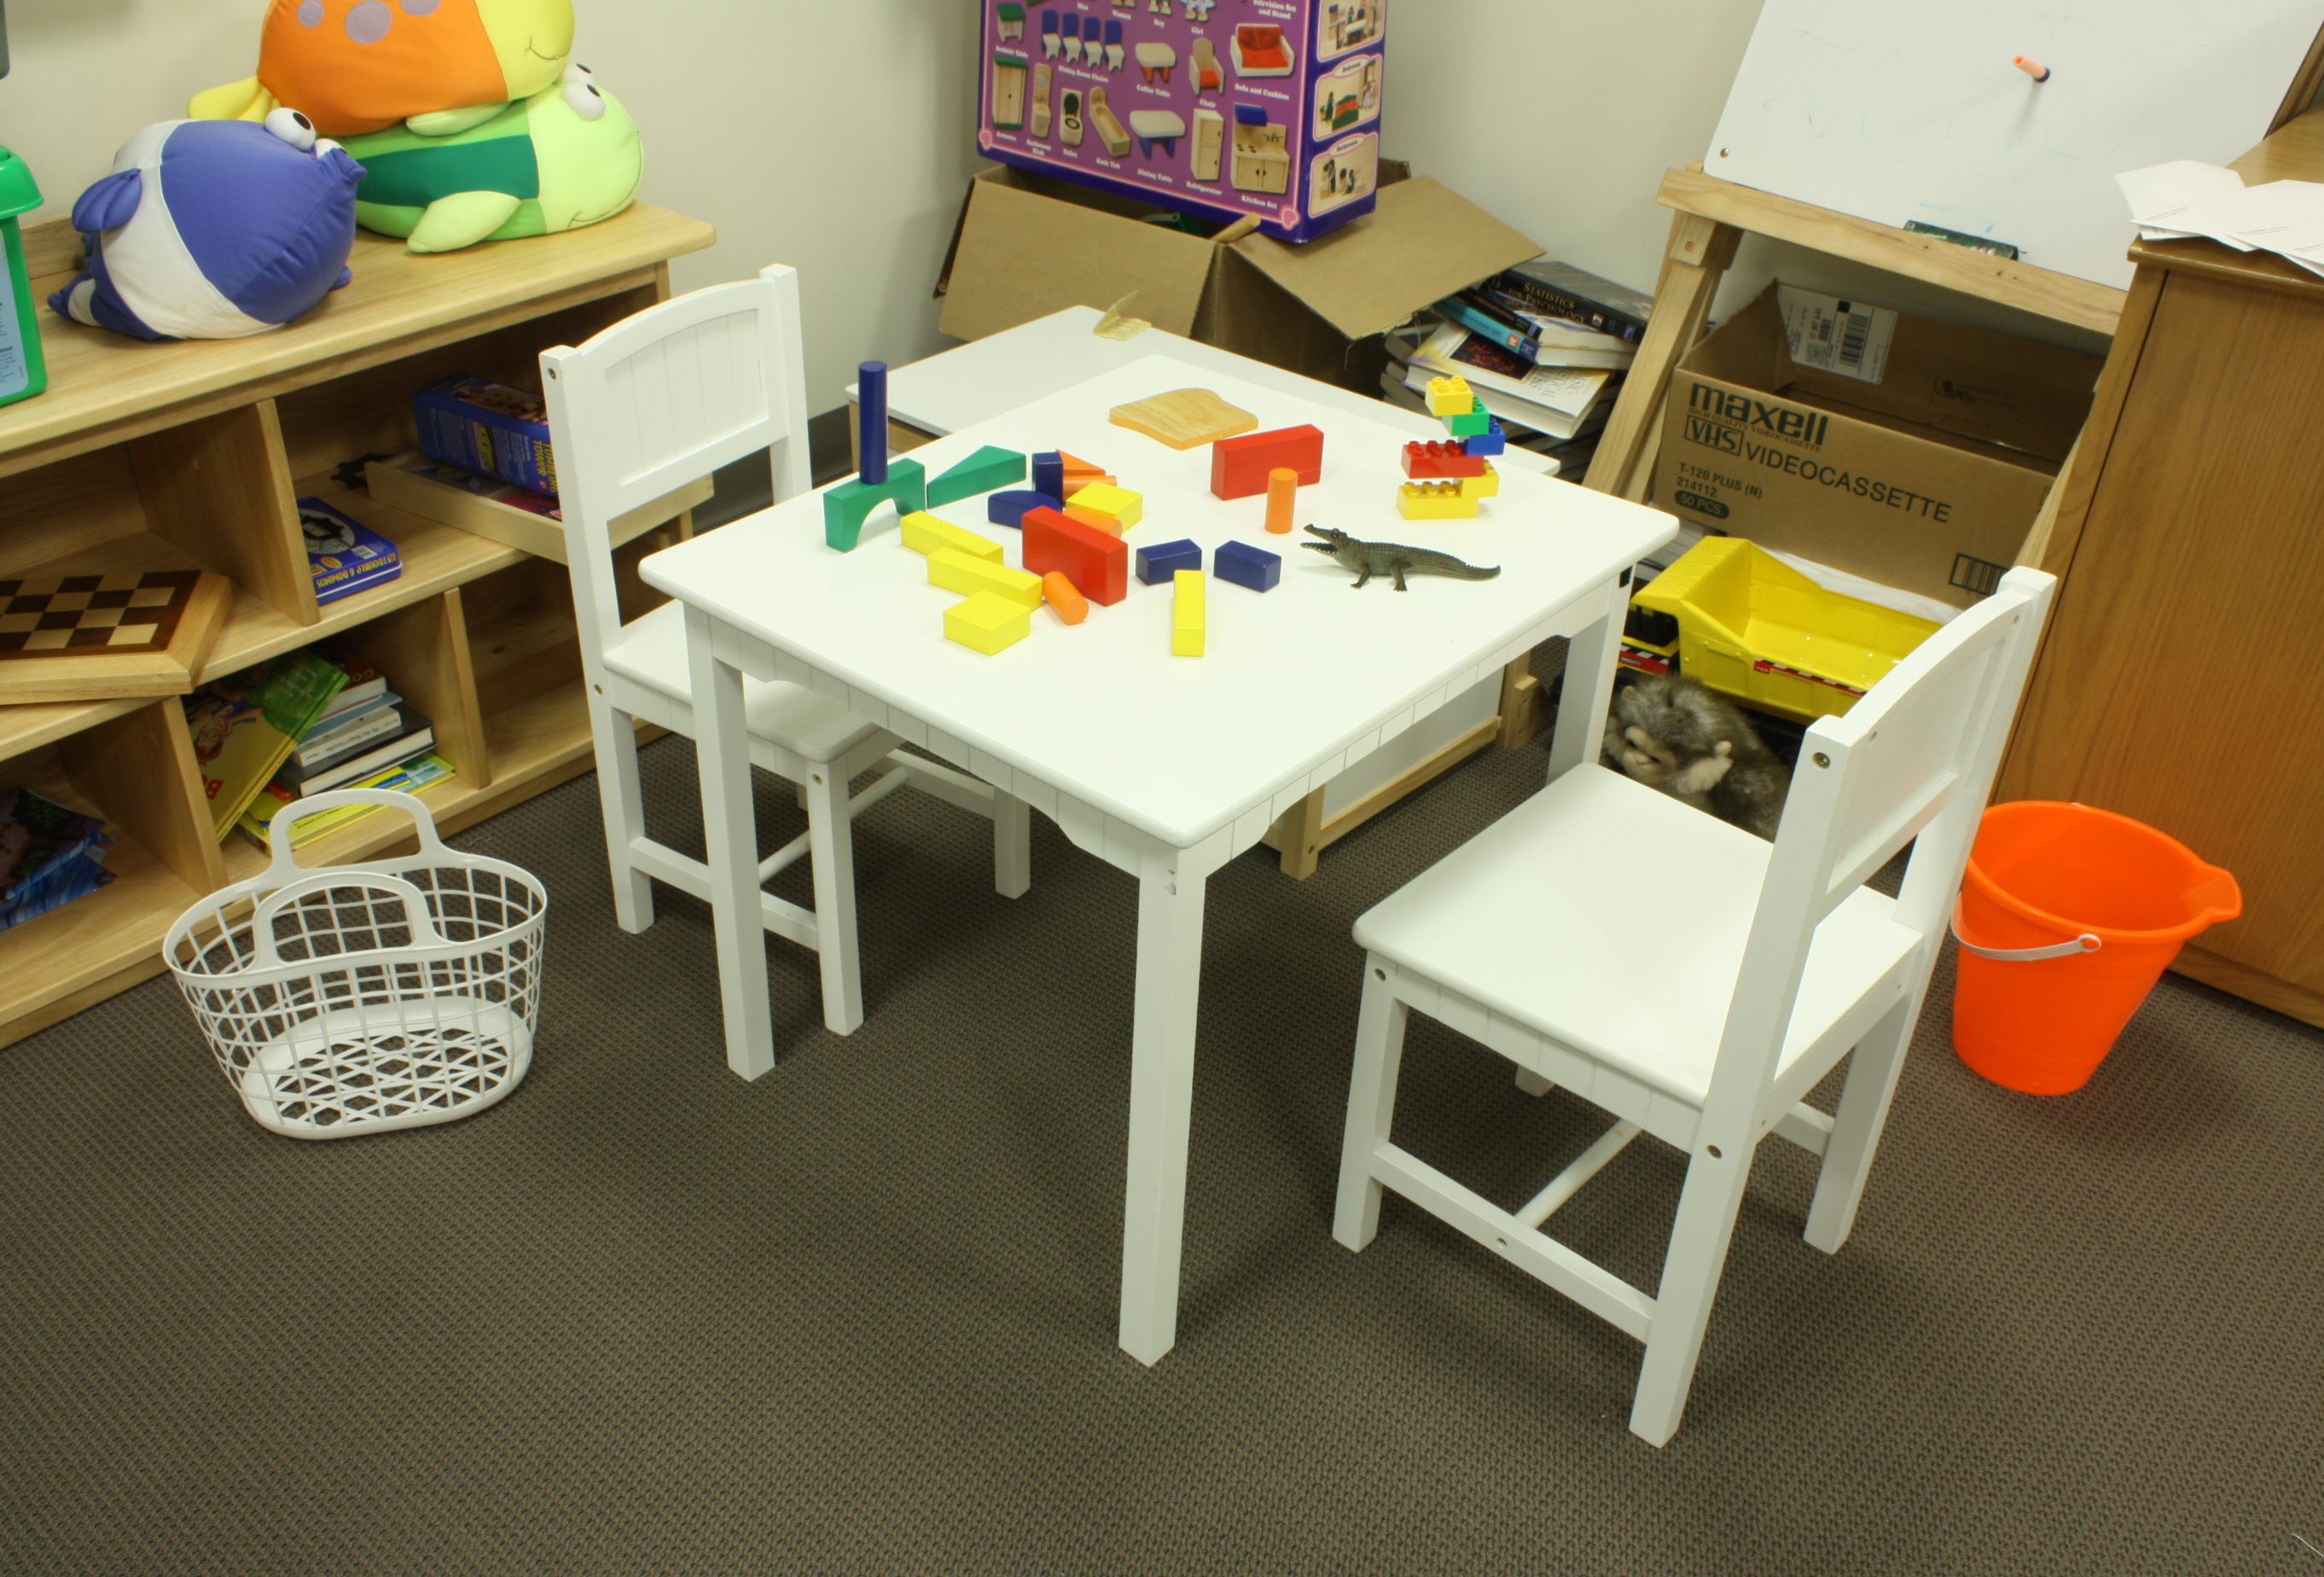
\includegraphics[width=0.4\textwidth, height= 5cm, keepaspectratio]{images/left-playtable-test.png}
 		\label{fig:test-matlab-left-02}
}
	\subfigure[Right RGB test image]{
 		 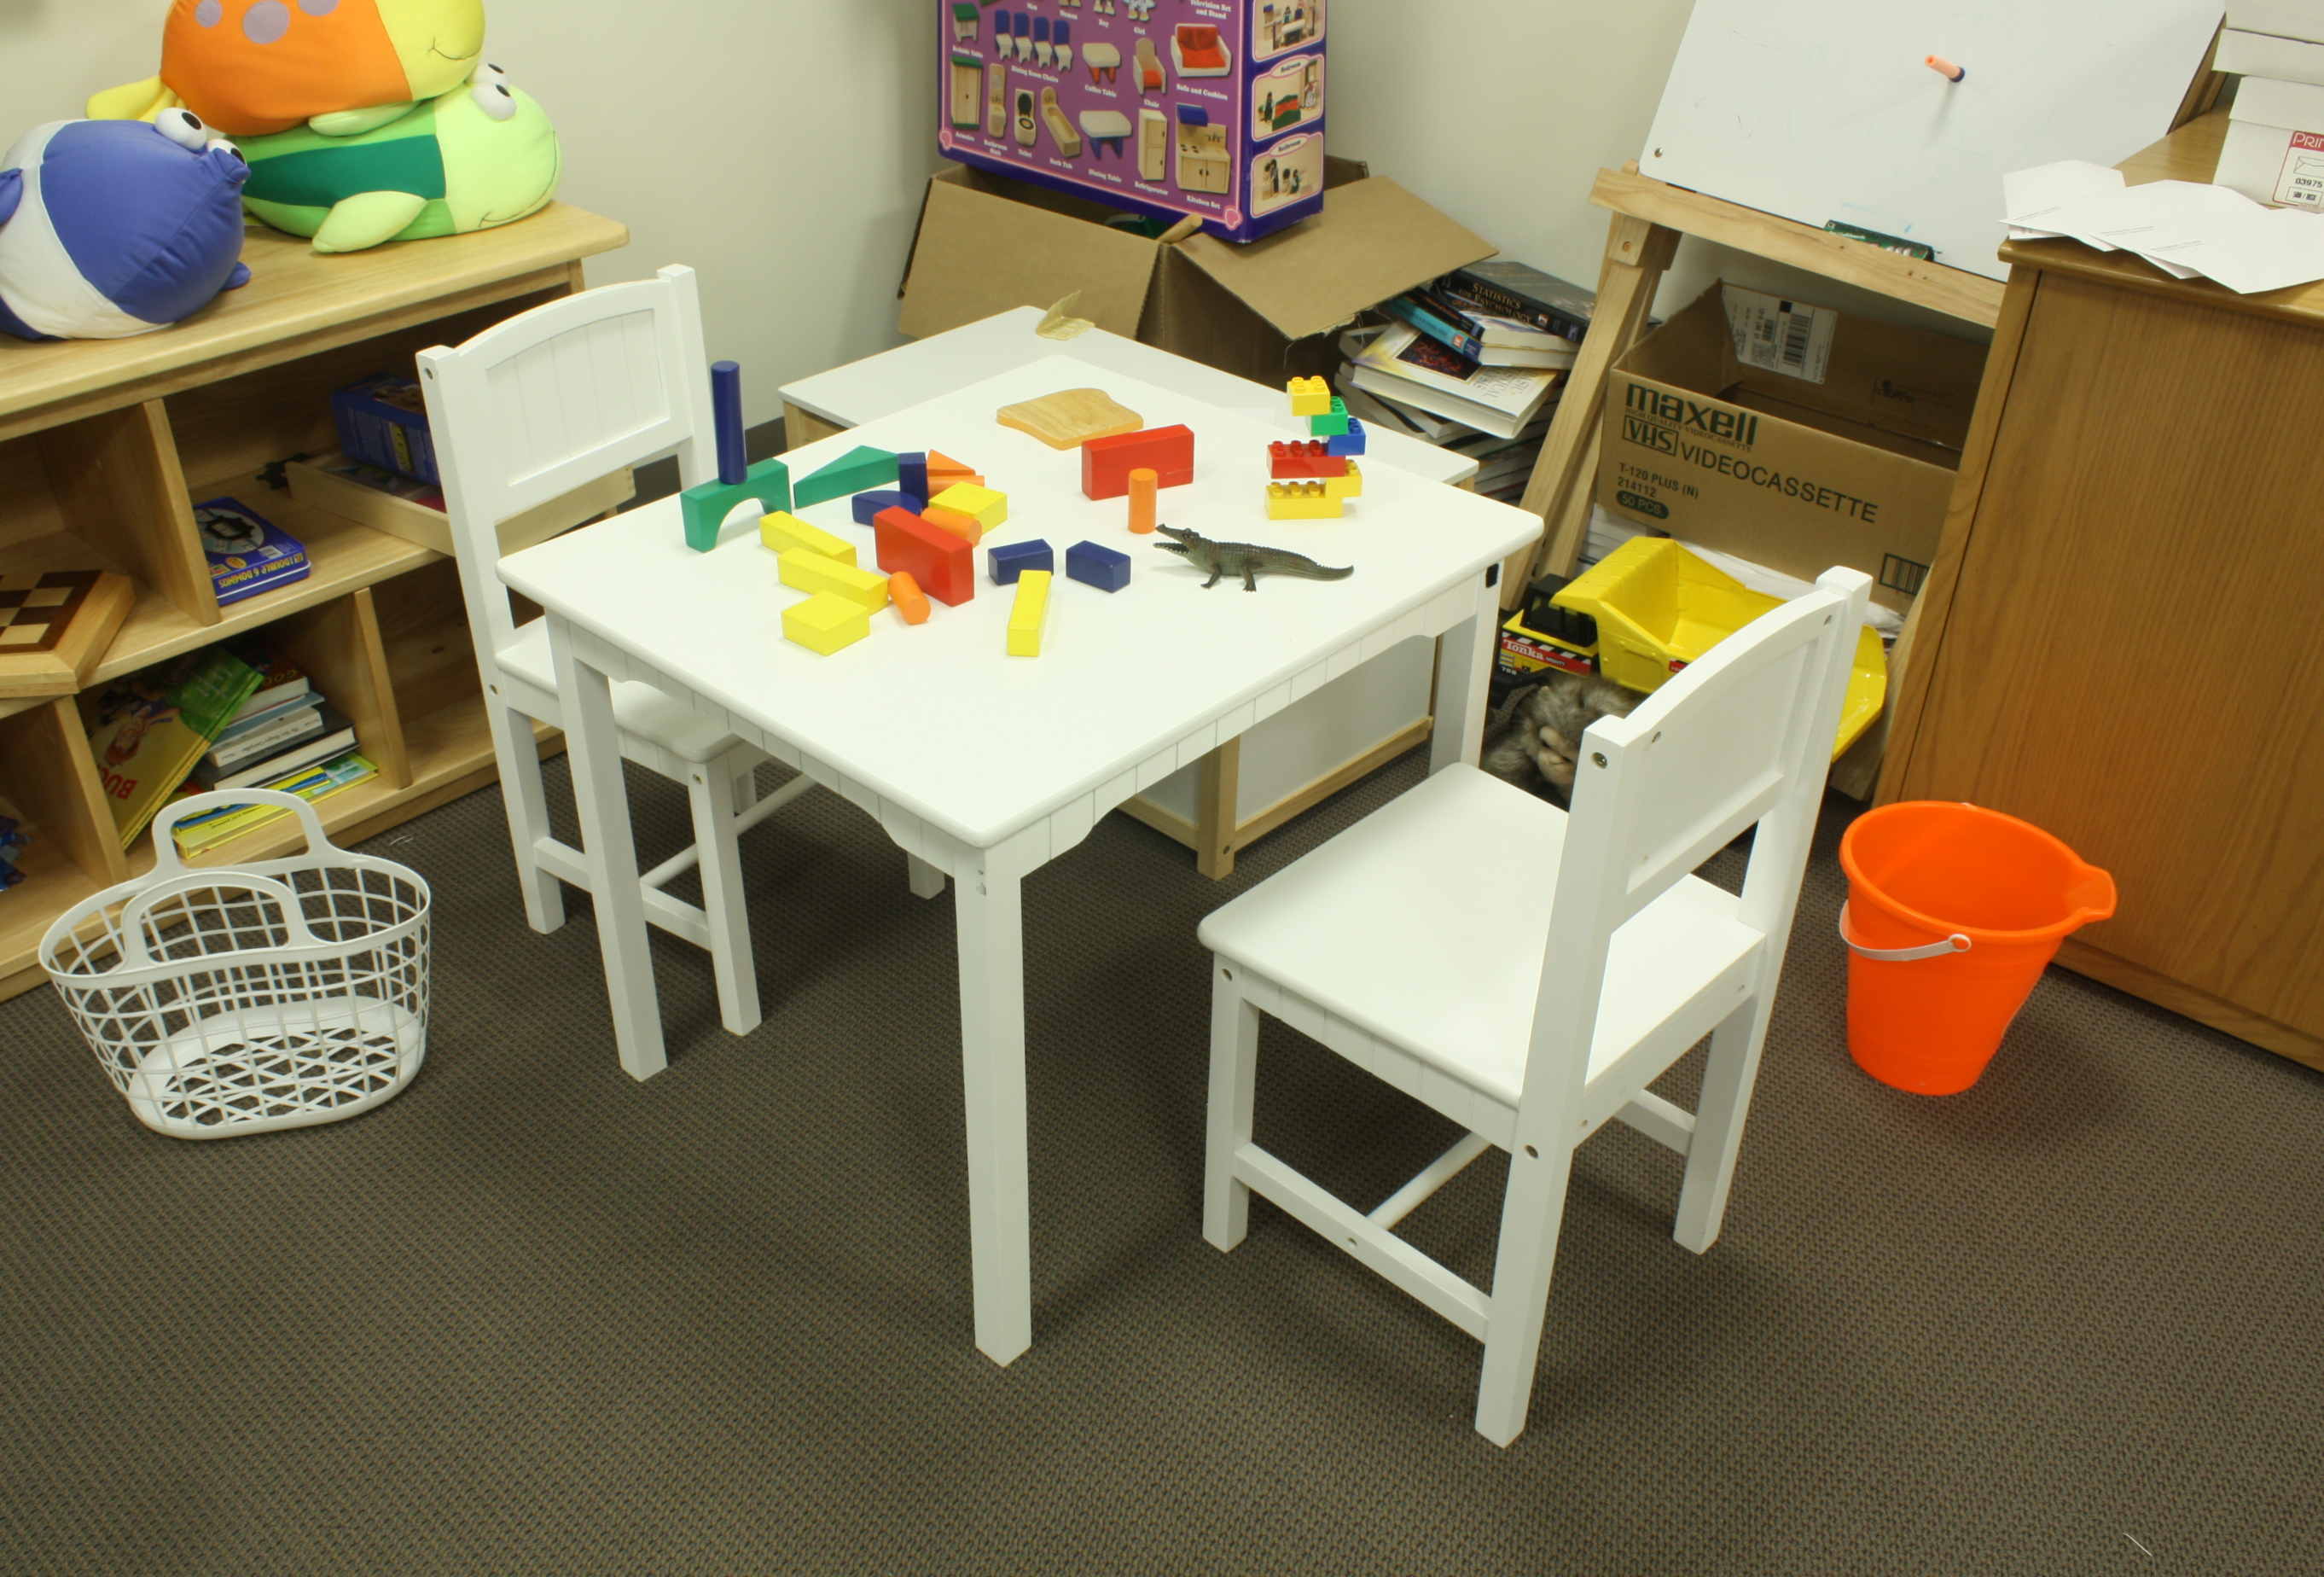
\includegraphics[width=0.4\textwidth, height= 5cm, keepaspectratio]{images/right-playtable-test.png}
 		 \label{fig:test-matlab-right-02}
}
	\subfigure[Disparity test image]{
	\includegraphics[width=0.8\textwidth, height=5cm, keepaspectratio]{images/disparity-map-playtable-test.png}
	\label{fig:disparity-test-02}
}
\caption{Test images from the Middlebury 2014 dataset with disparity image estimated with linear simple semi-global matching based method to test feasibility of thought strategy}
\label{fig:test-matlab-02}
\end{figure}

Figure~\ref{fig:test-matlab-02} displays the result of the estimation of a disparity image exploiting a stereo pair from the Middlebury 2014 dataset.
The disparity map shown in Figure~\ref{fig:disparity-test-02} has been achieved applying a rather simple and linear implementation of a semi-global based method, where information from an initial simulated sparse grid of point is employed.
As a matter of fact, in that initial stage of the project designing, the overall performance was not taken into account.
The main focus was the feasibility of the procedure compared to standard SGM-based algorithms. 
In fact, the core of the algorithm computations stand in the matching cost phase, which is based on the center-symmetric Census transform and on the Hamming distance computation.
Then, the aggregation cost step is carried out only over the 4 main orthogonal directions.
Finally, a basic left-right consistency check procedure is applied, which generate the lost of information of the two image sides.
Clearly, this behaviour is related to the disparity range employed in the algorithm.\\

\section{Derivative method results}
\label{section:der-method-results}

\begin{figure}[t]
	\centering
	\subfigure[Derivative-based method]{
 		\includegraphics[width=0.4\textwidth, height= 5cm, keepaspectratio]{images/raw-disparity-playtable-test.png}
 		\label{fig:derivative-based-test-table}
}
	\subfigure[SGM-based method]{
 		 \includegraphics[width=0.4\textwidth, height= 5cm, keepaspectratio]{images/sgm-based-playtable-test.png}
 		 \label{fig:sgm-based-test-table}
}
	\subfigure[OpenCV stereoSGBM method]{
	 \includegraphics[width=0.8\textwidth, height= 5cm, keepaspectratio]{images/opencv-baseline-test-playtable.png}
 		 \label{fig:opencv-baseline-test-table}
}
\caption{Results of disparity images obtained with the disparity-based lightweight method, the SGM-based method and the baseline result from the openCV built-in method}
\label{fig:test-novel-methods-table-01}
\end{figure}

As Figure~\ref{fig:disparity-test-02} proved, it is possible to achieve reasonable results with the designed method.
However, the interest thing is that, the initial tests performed show that, exploiting a sparse enough grid of points, which carry information on their 3D positions, the overall implementation can be made faster.\\
Therefore, after the initial researching phase, the algorithm started to be implemented in C++, in order to have a faster execution with respect to MATLAB, employing functions from the OpenCV library.
In this regard, Figure~\ref{fig:test-novel-methods-table-01} presents the grayscale disparity image achieved by applying the two designed methods, the derivative-based one and the SGM-based one, and then the outcome of the openCV built-in method is proposed as baseline for a visual comparison.\\
Therefore, considering the results of the disparity image of the \textbf{Playtable} dataset, some thoughts can be formulated.
First of all, as expected, in the baseline result in Figure~\ref{fig:opencv-baseline-test-table} the object are more detailed.
This is, thus, highly visible where the object present small or thin features, as for the bag in the middle-left area of the image.
Moreover, with the \texttt{stereoSGBM} algorithm there is an higher accuracy for the regions close to edges. \\
However, it has to be pointed out that, even if the openCV method has a lower amount of \textit{local} noise, e.g. along the object edges, which are visibly clear, it is affected by higher amount of \textit{general} noise, especially in occluded or texture-less areas.
Regarding this detail, both of the results obtained with the designed algorithms present a lower accuracy along edges, highlighted by the \textit{hairy} contours, however the surfaces are in general smoother.
Let us consider the top of the table or of the chairs, or even the wall in the background, as an example.
In the results of Figures~\ref{fig:derivative-based-test-table} and \ref{fig:sgm-based-test-table} the black spots are not generated.
They are, most likely, due to the occlusions presents in the two stereo images, considering the table and the chairs, or they are generated in texture-less regions, as for the wall, for which it is known that they SGBM algorithm tends to fail.\\
More interesting results can be then visualized when taking into account the outcomes of the different algorithms obtained using images taken from the company device.
As a matter of fact, in this case, contrarily to the images from widely-used datasets, such as the Middlebury 2014, the KITTI 2012 and 2015, there could likely be calibration errors in the stereo pair.
This leads to a mismatch between the epipolar lines of the two images, which should be overlapped to the image scanlines, when using a rectified stereo pair. 
Therefore, this problem causes a complete failure of the normal Semi-Global Box Matching procedure, as Figure \textbf{reference bad sgm images} demonstrates.\\
On the other hand, the designed method, thanks to the information coming from the points grid, is able to recover from small mismatching errors.
This condition proves the suitability of such a method in various situations, making it appropriate for those situations in which errors, even if minimal, cannot be avoided. 
It is, in fact, well known that in most of the real environment conditions it is generally difficult to have stable and controlled conditions, especially for lighting and for the physical stability of the hardware. 
The latter requirement is then extremely important for the accuracy of the final result. 
For this reason, in every industrial and commercial device employed in 3D estimation, as could be LiDAR or standard camera based hardware, a strong attention is provided to the system setup. 
However, errors related to unpredictable events or to little software bugs can affect the further computations, which would exploit the device outcome. \\

\subsection{Consistency check over derivative computation}
\label{subsection:result-consistency-check}

\begin{figure}[t]
	\centering
	\subfigure[Consistency check for derivative calculation]{
 		\includegraphics[width=0.4\textwidth, height= 5cm, keepaspectratio]{images/consistency-check-for-deriv-moto.png}
 		\label{fig:consistency-check-moto-01}
}
	\subfigure[No consistency check for derivative calculation]{
 		 \includegraphics[width=0.4\textwidth, height= 5cm, keepaspectratio]{images/no-consistency-check-for-deriv-moto.png}
 		 \label{fig:no-consistency-check-moto-01}
}
\caption{Comparison between applying and not a consistency check procedure over the same image}
\label{fig:consistency-check-comparison-moto-01}
\end{figure}

During the algorithm designing a specific phase of the pipeline demonstrates to be extremely important. 
Specifically, it consists on the \textit{consistency check} performed during the derivative computation when running the algorithm exploiting the simulated grid of points.
Actually, this consistency check becomes relevant in proximity of the edges, where the magnitude of the $Z$ component of a derivative calculated between two points that belong to far objects, and thus cut by an occlusion, tends to explode.
Therefore, this will affect the estimation procedure, which will most likely carry out wrong values for the computations performed in those areas. \\
Figure~\ref{fig:consistency-check-comparison-moto-01} clearly demonstrate the different on the final result when the consistency check over the derivatives calculations is applied or not.
When the magnitudes of the derivatives evaluated for a specific points are not correctly adjusted, if a set threshold on the $Z$ components of the derivative vector is exceeded, the final disparity image will show a huge amount of noise, which is obviously related to incorrect estimations.
Figure~\ref{fig:no-consistency-check-moto-01} is the proof of that.
Contrarily, in Figure~\ref{fig:consistency-check-moto-01} a better disparity map is visualized, which comes out when the consistency check operations are carried out.\\
Therefore, since the tests performed over the dataset images and using a simulated point grid, the necessity of the derivative correction was proven to be a valuable, and yet fundamental, step to reach an accurate result.

\subsection{Different thresholds for edge intensity result comparison}
\label{subsection:soft-strong-edge-threshold}

\begin{figure}[t]
	\centering
	\subfigure[Utilization of unique threshold over the whole input grid]{
 		\includegraphics[width=0.4\textwidth, height= 5cm, keepaspectratio]{images/micro-device-result-no-double-threshold-edges.png}
 		\label{fig:single-threshold-micro-01}
}
	\subfigure[Utilization of multiple threshold for distinguish edge strength]{
 		 \includegraphics[width=0.4\textwidth, height= 5cm, keepaspectratio]{images/micro-device-result-yes-double-threshold-edges.png}
 		 \label{fig:multiple-threshold-micro-01}
}
\caption{Comparison between utilization of different thresholds distinguish edge strength}
\label{fig:threshold-soft-strong-edges-micro-01}
\end{figure}

Taking into account the results obtained employing the company device, some considerations can be performed in relation to useful improvements that have been implemented to the algorithm during its development. \\
A modification to the initial pipeline of the algorithm, which shows to give interesting improvement in the accuracy of the final 3D point cloud estimated, stands in the utilization of multiple threshold for the edge analysis.
Specifically, as visible in Figure~\ref{fig:single-threshold-micro-01}, utilizing a unique threshold for edge checking over the whole input cloud wrong estimations are generated.
These are depicted in Figure~\ref{fig:single-threshold-micro-01} by the outlier points and are particularly visible where there is not a strong difference in depth among neighbouring point, as it happens between the face of the statue and calibration board on the foreground.\\
On the contrary, when different cases have been implemented in relation to different types of edges, strong and soft, those outliers have gone away, as Figure~\ref{fig:multiple-threshold-micro-01} shows.




\section{Stereo-matching based method results}
\label{section:stereo-match-results}



\section{OpenCV method baseline results}
\label{section:opencv-baseline-results}

\section{Overall comparison of the outcomes}
\label{section:method-comparison}

 

% 
%\chapter{Discussion}
\label{chapter:discussion}


The predetermined main objective of this project was to estimate a 3D dense point cloud starting from an initial sparse set of points and a pair of stereo undistorted images.
Moreover, this overall algorithm should have been executed in real time, in order to be following embedded in a stereo device which has to be suitable for autonomous driving, automotive and object detection related purposes.
Therefore, tests for guaranteeing a potentiality for this type of usability have to be carried out. \\
Overall, this can be evaluated as a challenging work, also considering the different algorithms developed since the early nineties in this field, which is considered as one of the most researched areas in computer vision, especially nowadays.\\
Moreover, since the initial stages of the project, there was the need of studying and understanding the company device and, thus, find the optimal way to embed it in the algorithm pipeline.
Additionally a novel strategy has to be thought, making it suitable for the requirements of the uses cases identified and competitive with the current methods.
Furthermore, since the beginning there was the decision to focus on a standard approach, differently from most of the latest algorithms, which are based on deep learning techniques.  
This decision was made in order to do not encounter the problem of the domain shifting, that is the drop in accuracy that most of the CNN-based algorithms face when dealing with new type of environment, especially real ones, on which the network has not been trained~\cite{Poggi2019}.
Moreover, another factor that pushed for basing the algorithm on a more standard stereo matching strategy stands on the requirement of being able to embed the algorithm on a relatively small device.
As a matter of fact, one of the company goals is to join the market of single-user devices, designing a product that should be extremely compact.
Therefore, there would be quite infeasible to execute in it algorithms that requires a high computational cost, such as ones based on neural network structure.
As a matter of fact, in this latter case, pre-training should be developed over an expensive machine, facing again the problem of the environment shifting. \\
Thereby, in order to guarantee a generally accurate result in every possible situation, and for the task of embedding the algorithm on compact devices, the decision was to design a standard based and lightweight method, which would be able to ensure, at lest theoretically, a real-time execution.
Considering the whole work done, those tasks were overall achieved.
Surely, further improvements are needed for guaranteeing an extremely fast execution, while keeping a high level of accuracy.
Besides that, if the initial requirements and the different challenges faced during the project development are taken into account, the final result achieved can be considered as a reliable proof of the accomplishment of the initial objective defined.

\section{Overall discussion over the project developed}
\label{section:overall-discussion}

Considering the overall project designed and especially comparing the outcomes achieved with the results of the OpenCV based Semi-Global Box Matching (SGBM) algorithm, which has been used as the baseline, the work done certainly showed that the strategy adopted is actually feasible for the predetermined goals.\\
However, a certain lack in accuracy is visible.
Moreover, the initial pre-processing section of the algorithm should be slightly improved, first of all the calibration of the stereo device, which is still not perfect. 



\section{Drawbacks of the designed algorithm}
\label{section:algorithm-drawbacks}

The main advantage of the algorithm developed is that it is sensibly fast.
However, it also hold some side drawbacks, which do not affect its main execution, although they limit the possibility of getting perfect results.\\
As a matter of fact, the algorithm relies a lot on the initial set of points provided through the device, which is surely highly accurate, however it has a certain lack of performance in the detection of small objects.
As specified since the initial chapters, the input point cloud is sparse, thus to ensure the maximum coverage of the scene. 
However, this cannot simultaneously guarantee high performance in terms of accuracy for all the objects in the scene.
Therefore, a more related stereo-matching strategy could be employed for those areas, thus to reduce the amount of errors and enhance the overall smoothness and continuity of the final dense cloud.\\
Taking that into account, some approaches have been thought in order to improve the algorithm on that side.
An example would stand on an initial segmentation of the scene.
This will identify the different areas of the analysed environment, and for those regions on which the number of points is too low, a more pure SGM based strategy would be applied. 
In fact, the fundamental downside of the classical SGM method is that it is highly expensive, computationally speaking, especially when the disparity range and the image density increase.
Therefore, if the number of disparity levels cannot be reduced drastically, the other feature that can be tackled is the dimension of the analysed area.
Hence, if it is applied to small regions, i.e. the segmented areas of small objects, a final potentially real-time execution could be ensured.


\section{Further improvements and future work}
\label{section:further-improvements}




% 
%\chapter{Conclusions}
\label{chapter:conclusions}

In the previous chapter some considerations regarding the tasks initially assigned to this project and the final results achieved has been proposed.
In relation to that, it is appropriate to summarize here the main acknowledgements and observations concerning the developed Master's thesis.

\section{General and conclusive analysis}
\label{section:general-final-analysis}

As outlined in Chapter~\ref{chapter:discussion}, the predominant goal set at  the initial stages of the project designing was the development of a novel method aimed at generate a dense 3D point cloud starting from a relatively small cluster of sparse points, thus to accurately describe the analysed environment.\\
This would be then be suitable for several applications, at different level of integration, in the computer vision area, such as object detection, robot manipulation, autonomous driving, monitoring car driver macro physical conditions\footnote{as an example an interesting application is tracking the car driver behaviour, thus to enhance the response of the safety system of the car for unexpected situations.}.\\
This can be reasonably evaluated as not a simple objective to accomplish, also taking into account the multiple algorithms developed so far in this researching area.
Therefore, different strategies to tackle the problem have been conceived since the very beginning of the project. 
Moreover, lots of tests over the algorithms produced have been carried out, in order to have clear and visible responses about the followed path.\\
The final results achieved can be, then, measured as a appropriate and suitable realization of the predetermined goals.
Certainly, as mentioned in Chapter~\ref{chapter:discussion}, further improvements will be added to the current work, thus to make it useful for real time applications, while guaranteeing a high level of accuracy of the outcome.
However, especially regarding the \textit{lightweight} algorithm designed, it clearly prove that, first of all, a high level of accuracy can be accomplished by exploiting its main idea, as displayed by the results shown in Chapter~\ref{chapter:evaluation}
Secondly, through proper improvements of the code, aimed at increasing its execution, real time applications can be considered as feasible.\\
Therefore, the accomplishment of the initial task identified should be regarded as produced, taking into account the main researching aspect of the work carried out.
In relation to that, future improvements of the project have already been planned, thus to make it certainly competitive with the current state-of-the-art algorithm and suitable for the market requirements.




% Load the bibliographic references
% ------------------------------------------------------------------
% You can use several .bib files:
% \bibliography{thesis_sources,ietf_sources}
\bibliography{sources}


% Appendices go here
% ------------------------------------------------------------------
% If you do not have appendices, comment out the following lines
\appendix
\chapter{First appendix}
\label{chapter:first-appendix}


\begin{figure}[b]
	\begin{center}
		\AaltoLogoLarge{1}{!}{aaltoRed}
	\end{center}
\end{figure}



% End of document!
% ------------------------------------------------------------------
% The LastPage package automatically places a label on the last page.
% That works better than placing a label here manually, because the
% label might not go to the actual last page, if LaTeX needs to place
% floats (that is, figures, tables, and such) to the end of the 
% document.
\end{document}
















